%%%%%%%%%%%%%%%%%%%%%%%%%%%%%%%%%%%%%%%%%%%%%%%%%%%%%%%%%%%%%%%%%%%%%%%%%%%
\documentclass[12pt]{article}
\usepackage[left=1cm, right=1cm, top=1cm, bottom=1cm]{geometry}
\usepackage{graphicx}
\usepackage{algorithm}
\usepackage{algpseudocode}
\usepackage{amsthm}
\usepackage{verbatim}% To print as typed ignoring the LaTeX commands
\usepackage{pdfpages}
\usepackage{csvsimple}
\usepackage{graphicx}
\usepackage{epstopdf}
\usepackage{epsfig}
\usepackage{float}
\usepackage{graphicx}% Include figure files
%\usepackage{cite}
%\usepackage{rotating}% Include figure files
\usepackage{dcolumn}% Align table columns on decimal point
\usepackage{bm}% bold math
\usepackage{tabularx}
\usepackage{hyperref}
%\usepackage{mciteplus}
\usepackage[utf8]{inputenc}
\usepackage{amssymb}
\usepackage{subfigure}
\usepackage{amsmath}
\usepackage{multirow}
%\usepackage{multicol}
%\usepackage{booktabs}
\usepackage{xspace}
\usepackage{booktabs}
\usepackage{sidecap}   % sidecaptions
\usepackage{subfigure}
\usepackage{ulem} % strikeout
\usepackage{array}
\usepackage{xcolor}
\usepackage[titletoc]{appendix}
\usepackage{rotating}
\usepackage{lipsum}  
%\usepackage[utf8]{inputenc}
%\usepackage[T1]{fontenc}
\usepackage [english]{babel}
\usepackage [autostyle, english = american]{csquotes}
\usepackage{bm}
\MakeOuterQuote{"}
%%%%%%%%%%%%%%%%%%%%%%%%%%%%%%%
\setlength{\textwidth}{16.75cm}
\setlength{\textheight}{23.0cm}
\setlength{\oddsidemargin}{0.0cm}
\setlength{\evensidemargin}{0.0cm}
\setlength{\headheight}{0cm}
\setlength{\headsep}{0cm}
\setlength{\topmargin}{0.0cm}
\setlength{\footskip}{1.5cm}
\usepackage{listings}
\usepackage{xcolor}
\usepackage[thinc]{esdiff}
\definecolor{codegreen}{rgb}{0,0.6,0}
\definecolor{codegray}{rgb}{0.5,0.5,0.5}
\definecolor{codepurple}{rgb}{0.58,0,0.82}
\definecolor{backcolour}{rgb}{0.95,0.95,0.92}

\lstdefinestyle{mystyle}{
    backgroundcolor=\color{backcolour},   
    commentstyle=\color{codegreen},
    keywordstyle=\color{magenta},
    numberstyle=\tiny\color{codegray},
    stringstyle=\color{codepurple},
    basicstyle=\ttfamily\footnotesize,
    breakatwhitespace=false,         
    breaklines=true,                 
    captionpos=b,                    
    keepspaces=true,                 
    numbers=left,                    
    numbersep=5pt,                  
    showspaces=false,                
    showstringspaces=false,
    showtabs=false,                  
    tabsize=2
}

\lstset{style=mystyle}
%%%%%%%%%%%%%%%%%%%%%%%%%%%%%
\renewcommand{\baselinestretch}{1.3}
%\usepackage[style=numeric-comp,sorting=none]{biblatex}%<- specify style
%\addbibresource{ref.bib}

%%%%%%%%%%%%%%%%%%%%%%%%%%%
\begin{document}
\baselineskip 0.7cm
\title{\bf \color{blue}MATHEMATICAL PHYSICS LAB FILE}
\vskip 3cm
\author{Anurag Das \\ (COLLEGE ROLL No.: 2020phy1116)\\(UNIVERSITY ROLL No. : 20068567014) \and 
%Partner C Name \\ (Partner C Roll N0) \\
{\color{blue}S.G.T.B. Khalsa College, University of
Delhi, Delhi-110007, India.} }

\maketitle
\vskip 4cm
\begin{center}
{\it {\color{blue}Lab File Submitted to}}\\
Dr.Savinder Kaur and Mr. Sushil Kumar Singh \\

\end{center}

\pagenumbering{gobble}

\newpage
%\vskip 1cm

\pagenumbering{roman}
\abstract{Projectile motion is a topic that one studies in 11th standard, and was recently in limelight as media outlets sought to explain the physical aspect of Neeraj Chopra’s javelin throw that won him the gold. However, in both the former and latter case, friction (air drag) is omitted. Here, we try to find out the optimal angle for release of javelin taking air drag into account. Differential equations in two dimensions are formulated, taking air drag into account as a viscous force acting against the direction of motion, are then numerically solved using rk2, rk4 and euler methods. When results are plotted, it is observed that 38° (using all the 3 methods) is the optimal angle for maximizing the horizontal range. This helps to understand why athletes throw javelins with a release angle in the late 30s, instead of 45°, which is theoretically the optimal angle for maximizing the range.}

%\abstract{\lipsum[1-1]}
\newpage
\tableofcontents
\newpage

\pagenumbering{arabic}
\section{Introduction}
\label{sec:intro}
The motivation for taking up this topic stems from our common passion for sports and physics. In late august this year, Indian athlete Neeraj Chopra won what was only the second individual gold medal in India’s olympic history. But what won our hearts as sports fans also baffled us as physics students. Long since class 11th, the time when we first studied projectile motion, we’ve had a notion that a release angle of 45° is optimum to maximize the range of an object in projectile motion. However, this explainer\cite{ref1} in the Indian express claimed otherwise. Therefore, we used this project as an opportunity to explore the frictional forces in play that we must take into account to conclude a more realistic optimum angle of release for maximizing the horizontal range of an object under projectile motion. Therefore, the project explores motion of a javelin as an object in projectile motion taking frictional forces into account as viscous force acting against the direction of motion. \\
An object that is in flight after being thrown or projected is called a projectile. Such a projectile might be a football, a cricket ball, a baseball or any other object. The motion of a projectile may be thought of as the result of two separate, simultaneously occurring components of motions. One component is along a horizontal direction without any acceleration and the other along the vertical direction with constant acceleration due to the force of gravity. Now when we include the force experienced due to air drag, we assume it as a basic force of nature with a universal form, but rather, it is an approximate model of the physics of viscous flow, with no one expression being accurate for all velocities. We know it always opposes motion, which means it is in a direction opposite to that of the velocity. A simple model for air resistance assumes that the frictional force is proportional to (negative of) the square of the projectile’s speed \cite{ref5}.  \\
Another important aspect of our project is the conversion of second order differential equations into first order ones. This involves producing two simultaneous first order differential equations. For example, if we have an equation $\frac{d^2x}{dt^2} = F(t,x)$, then it can be easily broken down into two simultaneous equations as $\frac{dx}{dt} = v$ and $\frac{dv}{dt} = F(t,x)$. In this way we'll get two equations for each dimension, and since we are talking about projectile motion in 2 dimensions, we will get a 2 pairs for first order simultaneous differential equations to solve, which means 4 in total. This means a little more work for us, but not too much for the computer, as we'll have to extend our ODE solver to solve 4 ODEs simultaneously.
First we introduce the theory of the topic, and also the frictional forces that we are taking into account. This is followed by the derivation of a combination of differential equations. This is followed by a short explainer on how to reduce a second order differential equation into two first order differential equations. The methodology section then explains about the tools and the numerical methods we have used in this project, followed by the algorithms of the numerical methods. So in this section we talk about python, the language we have used to code our algorithms, GNU Plot, our primary tool to plot any graphical results we have deduced, and rk2 and euler method. Euler and rk2 are the methods that we have used to numerically solve the differential equations we developed in the theory section. And then finally we move on to our results and analysis part. Here we analyse the results that we have plotted and also see if we can conclude a more realistic angle of release of an object in projectile motion in order to maximize the horizontal range. Moreover, we also see how these differ with and without friction. 
\newpage
%Cite a paper as\cite{PhysRev.47.777}
%%%%%%%%%%%%%%%%%%%%%%%%%%%%%%%%%%%%%%%%%%%%%%%%
\section{Theory}
\label{sec:theory}
\subsection{Problem Statement}
The aim is to find the optimal angle for maximization of horizontal range for a object under motion, taking drag into account and approximating the object as a standard men's javelin. 
\subsection{Projectile Motion - An introduction:}
An object that is in flight after being thrown or projected is called a projectile. Such a projectile might be a football, a cricket ball, a baseball or any other object. The motion of a projectile may be thought of as the result of two separate, simultaneously occurring components of motions. One component is along a horizontal direction without any acceleration and the other along the vertical direction with constant acceleration due to the force of gravity. It was Galileo who first stated this independence of the horizontal and the vertical components of projectile motion in his Dialogue on the great world systems (1632).

In our discussion, we shall initially assume that the air resistance has negligible effect on the motion of the projectile, in order to obtain the angle of maximization of horizontal range to compare with our final result (that takes friction due to air into account). Suppose that the projectile is launched with velocity $v_0$ that makes an angle $\theta_0$ with the x-axis as shown in Fig.1. After the object has been projected, the acceleration acting on it is that due to gravity which is directed vertically downward:
\begin{align}
  \Vec{a} &= -g\textbf{\textbf{$\hat{j}$}}  
\end{align}
Or, 
\begin{align}
a_x &= 0 \\
a_y &= -g
\end{align}

The components of initial velocity $v_0$ are :
\begin{align}
    v_{0x} = v_{0}\cos\theta_0 \\
    v_{0y} = v_{0}\sin\theta_0
\end{align}
\begin{figure}[H]
    \centering
    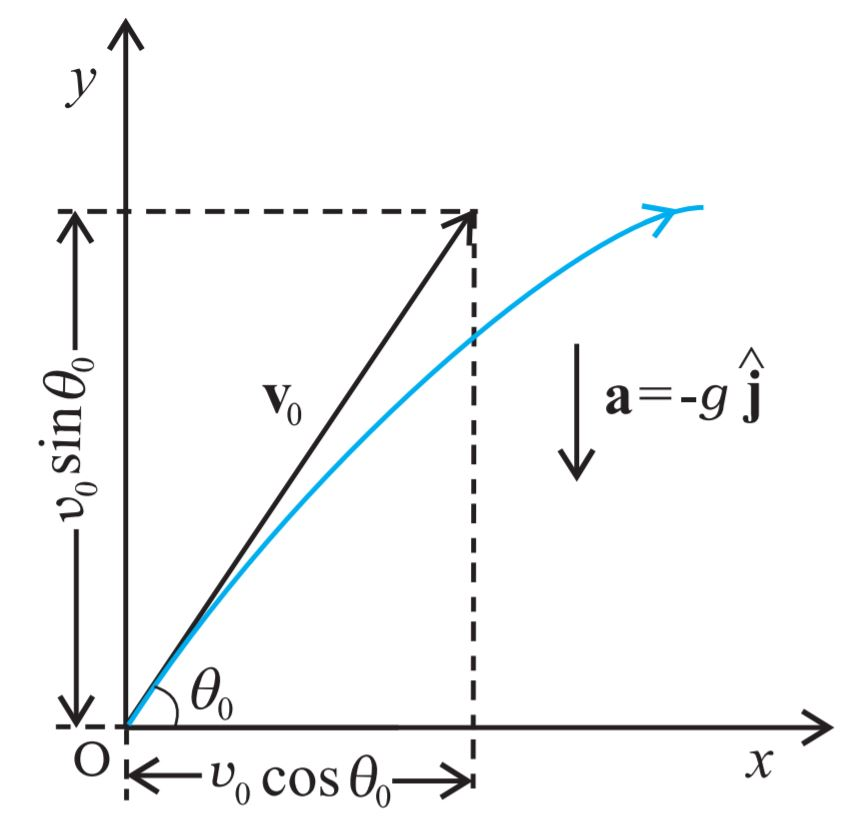
\includegraphics[width=0.5\textwidth]{fig1.JPG}
    \caption{Motion of an object projected with velocity $v_o$ at angle $\theta$ \cite{ref2}}
    \label{fig:fig1.JPEG}
\end{figure}
If we take the initial position to be the origin of the reference frame as shown in Fig. 1, we have : 
\begin{align*}
    x_o &= 0 \\
    y_o &= 0
\end{align*}
Then, by $y = y_o + v_{oy}t + \frac{1}{2}a_xt^2$ becomes : 
\begin{align}
x &= v_o \cos\theta_ot \\
y &= v_o \sin\theta_ot - \frac{g}{2t^2}    
\end{align}
The components of velocity at time t can be obtained using $v_y = v_{oy} + a_yt$:
\begin{align}
    v_x &= v_{ox} = v_o \cos \theta_o \\
    v_y &= vo \sin \theta_o - gt
\end{align}
Equation 6 and 7 give the $x$, and $y$ coordinates of the position of a projectile at time $t$ in terms of two parameters — initial speed $v_o$ and projection angle $\theta_o$ . Notice that the choice of mutually perpendicular $x$, and $y$ directions for the analysis of the projectile motion has resulted in a simplification. One of the components of velocity, i.e. $x$ component remains constant throughout the motion and only the y component changes, like an object in free fall in vertical direction. This is shown graphically at few instants in Fig. 2. Note that at the point of maximum height, $v_y = 0$ and therefore,
$$\theta = \tan^{-1} \frac{v_y}{v_x} = 0$$
\subsection{Equation of path of projectile}
What is the shape of the path followed by the projectile? This can be seen by eliminating the time between the expressions for $x$ and $y$ as given in 6 and 7. We obtain:
\begin{align}
    y = (\tan\theta_o)x - \frac{g}{2(v_o\cos\theta_o)^2}x^2
\end{align}
Now, since $g$, $\theta_o$ and $v_o$ are constants, Eq. 10 is of the form $y = ax + bx^2$, in which a and b are constants. This is the equation of a parabola, i.e. the path of the projectile is a parabola (Fig. 2).
\begin{figure}[H]
    \centering
    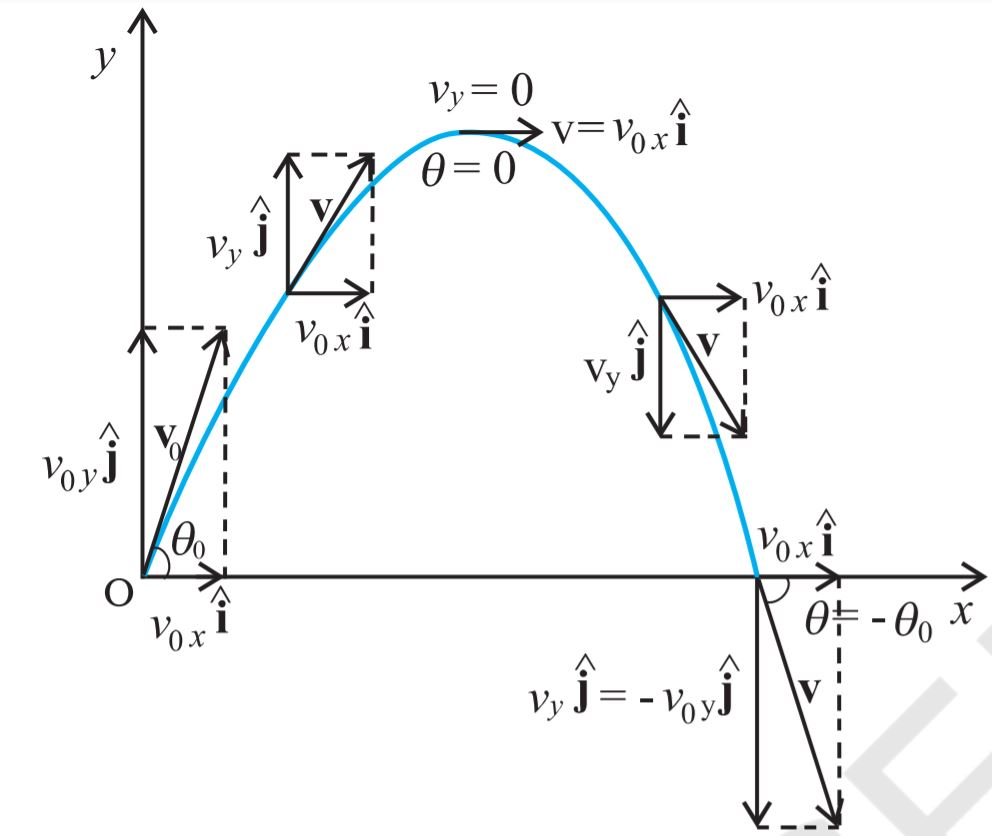
\includegraphics[width=0.66\textwidth]{fig2.JPG}
    \caption{Path of a projectile is a parabola \cite{ref3}}
    \label{fig:fig2.JPEG}
\end{figure}
\subsection{Time of maximum height}
Let the time take by the projectile to reach the maximum height be $t_m$. At this point $v_y = 0$, so we have from Eq. 8 and 9, $$v_y = v_0\sin\theta_o - gt_m = 0$$
Or, 
\begin{align}
    t_m = v_o\sin\theta_o/g
\end{align}
Total time $T_f$ during which the projectile is in flight can be obtained by putting $y = 0$ in Eq. 9. We get:
\begin{align}
    T_f = v_o\sin\theta_o/g
\end{align}
$T_f$ is known is known as the \textbf{Time of flight} of the projectile. We note that $T = 2t_m$, which is expected because of the symmetry of the parabolic path.
\subsection{Horizontal Range of the projectile}
The horizontal distance travelled by a projectile from its initial position to the position where it passes $y = 0$ during its fall is called the horizontal range, R. It is the distance travelled during the time of flight $T_f$ . Therefore, the range R is
$$R = (v_o \cos\theta_o)(T_f)$$ $$R = (v_o\cos\theta_o)(2v_o\sin\theta_o)/g$$
Or,
\begin{align}
    R = \frac{v^2_o\sin 2\theta_o}{g}
\end{align}
Equation 13 shows that for a given projection velocity $v_o$ , R is maximum when $\sin 2\theta_o$ is maximum, i.e., when $\theta_o = 45^{\circ}$.
\subsection{Differential equation and inclusion of air drag}
We want to determine if the inclusion of air resistance leads to a different optimal angle for maximization of the horizontal range. The basic physics is Newton’s second law in two dimensions for a frictional force $\Vec{f}$ opposing motion, and a vertical gravitational force $-g\textbf{\textbf{$\hat{j}$}}$
$$\Vec{f} - mg\hat{j} = m\frac{d^2\Vec{r}}{dt^2}$$
Now this can be broken down into 
\begin{align*}
    f_x &=  m\frac{d^2x}{dt^2}\\
    f_y - mg &= m\frac{d^2y}{dt^2}
\end{align*}
The force of friction $\Vec{f}$ is not a basic force of nature with a universal form, but rather, it is an approximate model of the physics of viscous flow, with no one expression being accurate for all velocities. We know it always opposes motion, which means it is in a direction opposite to that of the velocity. A simple model for air resistance assumes that the frictional force is proportional to square of the projectile’s speed, for high velocities like javelin's. 
$$\Vec{f} = -k|v_o|\Vec{v_o}$$
Where, $$\Vec{v_o} = v^2_{xo}\hat{i} + v^2_{yo}\hat{j}$$
$$|v_o| = \sqrt{v^2_{xo} + v^2_{yo}}$$
Which can be broken down, and simplified, after taking $v_x = |v|\cos\theta_o$, and $v_y = |v|\sin\theta_o$ as:
\begin{align}
   f_x &= -k|v_o|^2\cos\theta_o \\
   f_y &= -k|v_o|^2\sin\theta_o
\end{align}

\subsection{Conversion of 2nd order ODEs to simultaneous 1st order ODEs}
Now, what have obtained our second order equation. However, we can convert then into first order ones, and then apply the numerical methods we desire. That we would lead to production of 1st order ODEs for each second order ODE. Moreover, since we have 2 second order ODEs, we will, in total, have 4 ODEs. 

Now we pick a 4D vector $\Vec{Y}$ as our dependent variable such that: $$\Vec{Y} = Y_1\hat{e}_1 + Y_2\hat{e}_2 + Y_3\hat{e}_3 + Y_4\hat{e}_4 $$
\begin{align}
    Y_1 &= x(t) \\
    Y_2 &= \frac{dx}{dt} \\
    Y_3 &= y(t) \\
    Y_4 &= \frac{dy}{dt}
\end{align}
Therefore, our equations finally turn out to be:
\begin{align}
    \frac{dY_0}{dt} \left(\equiv \frac{dx}{dt}\right) &= Y_1 \\
    \frac{dY_1}{dt} \left(\equiv \frac{d^2x}{dt}\right) &= \frac{f_x}{m} \\
    \frac{dY_2}{dt} \left(\equiv \frac{dy}{dt}\right) &= Y_3 \\
    \frac{dY_3}{dt} \left(\equiv \frac{d^2y}{dt}\right) &= \frac{f_y}{m} - g 
\end{align}
\newpage

\subsection{Initial values provided to the python program}
Here are all the initial values we provided to the program:
\begin{itemize}
    \item $Y_0 \,(\equiv x_o) = 0$ m
    \item $Y_1 \,(\equiv \frac{dx_o}{dt}) = 29\cos\theta_o$ m/s \cite{ref11}
    \item $Y_2 \,(\equiv y_o) = 2$ m (an extensive explanation of this has been done in the analysis section)
    \item $Y_3 \,(\equiv \frac{dx_o}{dt}) = 29\sin\theta_o$ m/s \cite{ref12}
    \item k = 0.00470625 kg/m (This is explained in appendix section C)
\end{itemize}
Since all these values are in SI units, the dimensions from the LHS and RHS will get cancelled from each side of the differential equation, and we will get a dimensionless equation to solve, as:
\begin{enumerate}
    \item LHS of (20) and (22) are the rates of change of $Y_0$ and $Y_2$, which means that are the rates of the change of $x$ and $y$ co-ordinates respectively, which means velocity. In the RHS of these equations we have  $Y_1$ and  $Y_3$ respectively, which are the velocities provided in the $x$ and $y$ direction respectively. Therefore, (20) and (22) are dimensionally correct which will yield are dimensionless equation as units on both sides will cancel out.
    \item Similarly, LHS of (21) and (22) are the rates of change of $Y_1$ and $Y_3$, which means that are the rates of the change of $v_{ox}$ and $v_{oy}$ respectively, which means acceleration. In the RHS of these equations we have  $\frac{f_x}{m}$ and  $\frac{f_y}{m} - g$ respectively, acceleration (or retardation) they will face will in the respective axis. Therefore, (21) and (23), too, are dimensionally correct which will yield are dimensionless equation as units on both sides will cancel out. Note that $\frac{f_x}{m}$ and  $\frac{f_y}{m}$ mean that we are dividing force(s) by mass, which gives acceleration.
\end{enumerate}
\newpage
%%%%%%%%%%%%%%%%%%%%%%%%%%%%%%%%%
\section{Methodology}
\label{sec:method}
\subsection{List of tools used}
Following are the list of tools that we used to make this project, which includes writing programs, running simulations, plotting graphs, writing reports, and making beamers:
\begin{itemize}
    \item Python (through Google Colab)
    \item GNU plot (through GNU Plot 5.2, and Overleaf)
    \item \LaTeX \,(through Overleaf)
\end{itemize}
\subsection{Numerical Methods, and Algorithms}
    Numerical methods for ODE are methods used to find numerical approximations to the solutions of ODE. Numerical methods prove to be useful when one is able to prove the existence of the solution theoretically without being able to obtain its analytical form,  at this moment, one usually turns to the numerical methods to get an approximation of the solution. Numerical methods we used here are: Euler method, Range-Kutta 2nd order, Range-Kutta 4th order. 
%%%%%%%%%%%%%%%%%%%%%%%%%%%%%%%%%%%%%%%%%%%%%%%%%%%%%%%
    \subsubsection{Euler Method}
    \begin{algorithm}[H]
  \caption{Euler Method}
  \begin{algorithmic}
    \Procedure{Euler}{$x_o, t_i, t_f, N$}\\
    \Comment Let the differential equation be $dx/dt = f(t,x)$ and for the initial conditions $t=t_o$, we have $x=x_o$
    \State $h \gets (t_f - t_i)/N$
     \For{\texttt{$i$ in $(0,N)$}}
        \State \texttt{$x_{i+1} \gets x_i + h*f(t_i, x_i)$}
      \EndFor
    \EndProcedure
  \end{algorithmic}
\end{algorithm}
%%%%%%%%%%%%%%%%%%%%%%%%%%%%%%%%%%%%%%%%%%%%%%%%%%%%%%%%%
    \subsubsection{RK2 Method}
    \begin{algorithm}[H]
  \caption{RK2 Method}
  \begin{algorithmic}
    \Procedure{rk2}{$x_o, t_i, t_f, N$}\\
    \Comment Let the differential equation be $dx/dt = f(t,x)$ and for the initial conditions $t=t_o$, we have $x=x_o$
    \State $h \gets (t_f - t_i)/N$
     \For{\texttt{$i$ in $(0,N)$}}
     \State $K_1 \gets h*f(t_i, x_i)$
     \State $K_2 \gets h*f(t_i + h, x_i + K_1)$
        \State \texttt{$x_{i+1} \gets x_i + \frac{K_1 + K_2}{2}$}
      \EndFor
    \EndProcedure
  \end{algorithmic}
\end{algorithm}
%%%%%%%%%%%%%%%%%%%%%%%%%%%%%%%%%%%%%%%%%%%%%%%%%%%%%%%%%
    \subsubsection{RK4 Method}
    \begin{algorithm}[H]
  \caption{RK4 Method}
  \begin{algorithmic}
    \Procedure{rk4}{$x_o, t_i, t_f, N$}\\
    \Comment Let the differential equation be $dx/dt = f(t,x)$ and for the initial conditions $t=t_o$, we have $x=x_o$
    \State $h \gets (t_f - t_i)/N$
     \For{\texttt{$i$ in $(0,N)$}}
     \State $K_1 \gets f(t_i, x_i)$
     \State $K_2 \gets f(t_i + \frac{h}{2}, x_i + h*\frac{K_1}{2})$
     \State $K_3 \gets f(t_i + \frac{h}{2}, x_i + h*\frac{K_2}{2})$
     \State $K_4 \gets f(t_i + h, x_i + h*K_3)$
     \State $K_{RK4} \gets \frac{K_1 + 2K_2 + 2K_3 + K_4}{6}$
        \State \texttt{$x_{i+1} \gets x_i + h*K_{RK4}$}
      \EndFor
    \EndProcedure
  \end{algorithmic}
\end{algorithm}
%%%%%%%%%%%%%%%%%%%%%%%%%%%%%%%%%%%%%%%%%%%%%%%%%%%%%%%%%%
\newpage
\subsection{Limitations}
\begin{itemize}
    \item All these methods provide an approximate solution to the differential equation and not exact.
    \item Numerical methods to solve differential equations are often very lengthy and are solved using computers, and to get fairly accurate results, they sometimes may require high computational power.

\end{itemize}
\newpage
%%%%%%%%%%%%%%%%%%%%%%%%%%%%%%%%%%%%%%
\section{Analysis of Numerical Results}
\begin{figure}[H]
    \centering
    % GNUPLOT: LaTeX picture with Postscript
\begingroup
  % Encoding inside the plot.  In the header of your document, this encoding
  % should to defined, e.g., by using
  % \usepackage[cp1252,<other encodings>]{inputenc}
  \inputencoding{cp1252}%
  \makeatletter
  \providecommand\color[2][]{%
    \GenericError{(gnuplot) \space\space\space\@spaces}{%
      Package color not loaded in conjunction with
      terminal option `colourtext'%
    }{See the gnuplot documentation for explanation.%
    }{Either use 'blacktext' in gnuplot or load the package
      color.sty in LaTeX.}%
    \renewcommand\color[2][]{}%
  }%
  \providecommand\includegraphics[2][]{%
    \GenericError{(gnuplot) \space\space\space\@spaces}{%
      Package graphicx or graphics not loaded%
    }{See the gnuplot documentation for explanation.%
    }{The gnuplot epslatex terminal needs graphicx.sty or graphics.sty.}%
    \renewcommand\includegraphics[2][]{}%
  }%
  \providecommand\rotatebox[2]{#2}%
  \@ifundefined{ifGPcolor}{%
    \newif\ifGPcolor
    \GPcolortrue
  }{}%
  \@ifundefined{ifGPblacktext}{%
    \newif\ifGPblacktext
    \GPblacktextfalse
  }{}%
  % define a \g@addto@macro without @ in the name:
  \let\gplgaddtomacro\g@addto@macro
  % define empty templates for all commands taking text:
  \gdef\gplbacktext{}%
  \gdef\gplfronttext{}%
  \makeatother
  \ifGPblacktext
    % no textcolor at all
    \def\colorrgb#1{}%
    \def\colorgray#1{}%
  \else
    % gray or color?
    \ifGPcolor
      \def\colorrgb#1{\color[rgb]{#1}}%
      \def\colorgray#1{\color[gray]{#1}}%
      \expandafter\def\csname LTw\endcsname{\color{white}}%
      \expandafter\def\csname LTb\endcsname{\color{black}}%
      \expandafter\def\csname LTa\endcsname{\color{black}}%
      \expandafter\def\csname LT0\endcsname{\color[rgb]{1,0,0}}%
      \expandafter\def\csname LT1\endcsname{\color[rgb]{0,1,0}}%
      \expandafter\def\csname LT2\endcsname{\color[rgb]{0,0,1}}%
      \expandafter\def\csname LT3\endcsname{\color[rgb]{1,0,1}}%
      \expandafter\def\csname LT4\endcsname{\color[rgb]{0,1,1}}%
      \expandafter\def\csname LT5\endcsname{\color[rgb]{1,1,0}}%
      \expandafter\def\csname LT6\endcsname{\color[rgb]{0,0,0}}%
      \expandafter\def\csname LT7\endcsname{\color[rgb]{1,0.3,0}}%
      \expandafter\def\csname LT8\endcsname{\color[rgb]{0.5,0.5,0.5}}%
    \else
      % gray
      \def\colorrgb#1{\color{black}}%
      \def\colorgray#1{\color[gray]{#1}}%
      \expandafter\def\csname LTw\endcsname{\color{white}}%
      \expandafter\def\csname LTb\endcsname{\color{black}}%
      \expandafter\def\csname LTa\endcsname{\color{black}}%
      \expandafter\def\csname LT0\endcsname{\color{black}}%
      \expandafter\def\csname LT1\endcsname{\color{black}}%
      \expandafter\def\csname LT2\endcsname{\color{black}}%
      \expandafter\def\csname LT3\endcsname{\color{black}}%
      \expandafter\def\csname LT4\endcsname{\color{black}}%
      \expandafter\def\csname LT5\endcsname{\color{black}}%
      \expandafter\def\csname LT6\endcsname{\color{black}}%
      \expandafter\def\csname LT7\endcsname{\color{black}}%
      \expandafter\def\csname LT8\endcsname{\color{black}}%
    \fi
  \fi
    \setlength{\unitlength}{0.0500bp}%
    \ifx\gptboxheight\undefined%
      \newlength{\gptboxheight}%
      \newlength{\gptboxwidth}%
      \newsavebox{\gptboxtext}%
    \fi%
    \setlength{\fboxrule}{0.5pt}%
    \setlength{\fboxsep}{1pt}%
    \definecolor{tbcol}{rgb}{1,1,1}%
\begin{picture}(8640.00,5760.00)%
    \gplgaddtomacro\gplbacktext{%
      \csname LTb\endcsname%%
      \put(1078,704){\makebox(0,0)[r]{\strut{}0}}%
      \put(1078,3624){\makebox(0,0)[r]{\strut{}59.8}}%
      \put(1078,4994){\makebox(0,0)[r]{\strut{}87.86}}%
      \put(1210,484){\makebox(0,0){\strut{}0$^\circ$}}%
      \put(4179,484){\makebox(0,0){\strut{}38$^\circ$}}%
      \put(4727,484){\makebox(0,0){\strut{}45$^\circ$}}%
      \put(8243,484){\makebox(0,0){\strut{}90$^\circ$}}%
    }%
    \gplgaddtomacro\gplfronttext{%
      \csname LTb\endcsname%%
      \put(209,2901){\rotatebox{-270}{\makebox(0,0){\strut{}$x_{max}$ (m)}}}%
      \put(4726,154){\makebox(0,0){\strut{}$\theta (^\circ)$}}%
      \csname LTb\endcsname%%
      \put(7256,4926){\makebox(0,0)[r]{\strut{}Without drag}}%
      \csname LTb\endcsname%%
      \put(7256,4706){\makebox(0,0)[r]{\strut{}With drag}}%
      \csname LTb\endcsname%%
      \put(4726,5429){\makebox(0,0){\strut{}EULER: Variation of $x_{max}$ with $\theta$}}%
    }%
    \gplbacktext
    \put(0,0){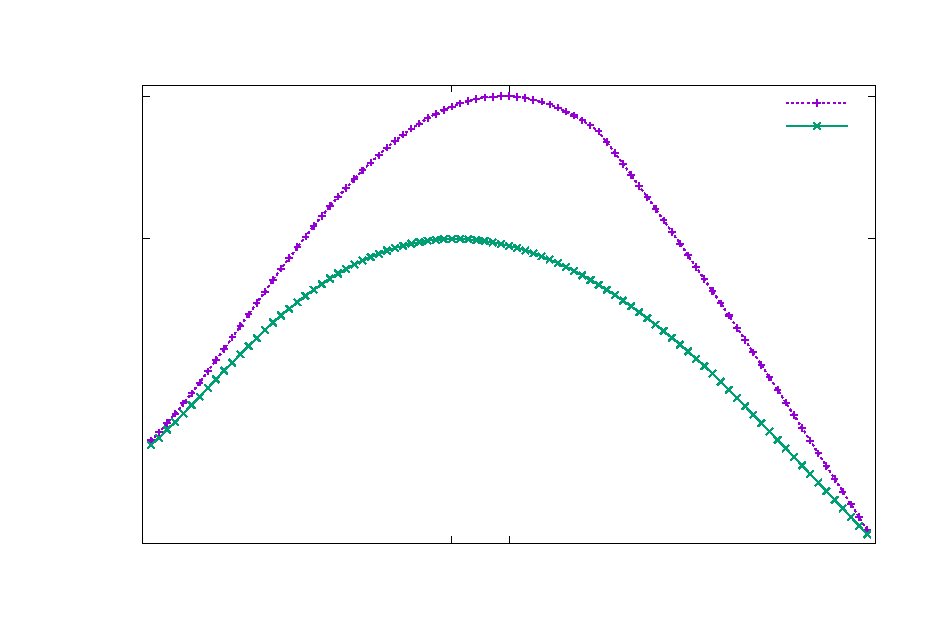
\includegraphics[width={432.00bp},height={288.00bp}]{EulerVariationTEX}}%
    \gplfronttext
  \end{picture}%
\endgroup

    \caption{Figure shows the variation of $x_{max}$ with $\theta$, computed using the Euler method}
    \label{fig:my_label2}
\end{figure}
\begin{itemize}
    \item The curve doesn’t start from 0 on the $y$ axis. This is because the initial value of coordinate was taken to be 2 meters (explanation will follow in the next set of graphs), and now it must be very intuitive to visualise that when you project something from a height at 0$^\circ$ and some initial velocity, it will travel to a non zero distance.
    \item Also, we see that the curve for the analysis done without drag gives the optimal angle for maximization of range to be 45$^\circ$. This was something we proved in the theory section too. 
    \item Now, the curve for the analysis done taking drag into account gives the optimal angle for maximization of range to be 38$^\circ$.
    \item This is near our initial figure of ~36$^\circ$, and might differ because that figure only pertains to a single person, Mr. Neeraj Chopra, and thus might be a result of some habits and some other customization beyond the scope of this project. 
    \item Moreover, we see that that the range doesn't vary very much from 35$^\circ$ to 45$^\circ$ as can be seen in Figure 1. The coefficient of variation in $x_{max}$ from 35$^\circ$ to 40$^\circ$ is 0.23\%.
    \item Therefore, we might conclude that it depends more on the players' execution of their craft than it does on the angle of launch. 
    \item Moreover, this source\cite{ref4} on the web verifies that the optimal angle for maximization of range was in the late 30s, and hence our result can be judged fairly good.
\end{itemize}
\begin{figure}[H]
    \centering
    % GNUPLOT: LaTeX picture with Postscript
\begingroup
  % Encoding inside the plot.  In the header of your document, this encoding
  % should to defined, e.g., by using
  % \usepackage[cp1252,<other encodings>]{inputenc}
  \inputencoding{cp1252}%
  \makeatletter
  \providecommand\color[2][]{%
    \GenericError{(gnuplot) \space\space\space\@spaces}{%
      Package color not loaded in conjunction with
      terminal option `colourtext'%
    }{See the gnuplot documentation for explanation.%
    }{Either use 'blacktext' in gnuplot or load the package
      color.sty in LaTeX.}%
    \renewcommand\color[2][]{}%
  }%
  \providecommand\includegraphics[2][]{%
    \GenericError{(gnuplot) \space\space\space\@spaces}{%
      Package graphicx or graphics not loaded%
    }{See the gnuplot documentation for explanation.%
    }{The gnuplot epslatex terminal needs graphicx.sty or graphics.sty.}%
    \renewcommand\includegraphics[2][]{}%
  }%
  \providecommand\rotatebox[2]{#2}%
  \@ifundefined{ifGPcolor}{%
    \newif\ifGPcolor
    \GPcolortrue
  }{}%
  \@ifundefined{ifGPblacktext}{%
    \newif\ifGPblacktext
    \GPblacktextfalse
  }{}%
  % define a \g@addto@macro without @ in the name:
  \let\gplgaddtomacro\g@addto@macro
  % define empty templates for all commands taking text:
  \gdef\gplbacktext{}%
  \gdef\gplfronttext{}%
  \makeatother
  \ifGPblacktext
    % no textcolor at all
    \def\colorrgb#1{}%
    \def\colorgray#1{}%
  \else
    % gray or color?
    \ifGPcolor
      \def\colorrgb#1{\color[rgb]{#1}}%
      \def\colorgray#1{\color[gray]{#1}}%
      \expandafter\def\csname LTw\endcsname{\color{white}}%
      \expandafter\def\csname LTb\endcsname{\color{black}}%
      \expandafter\def\csname LTa\endcsname{\color{black}}%
      \expandafter\def\csname LT0\endcsname{\color[rgb]{1,0,0}}%
      \expandafter\def\csname LT1\endcsname{\color[rgb]{0,1,0}}%
      \expandafter\def\csname LT2\endcsname{\color[rgb]{0,0,1}}%
      \expandafter\def\csname LT3\endcsname{\color[rgb]{1,0,1}}%
      \expandafter\def\csname LT4\endcsname{\color[rgb]{0,1,1}}%
      \expandafter\def\csname LT5\endcsname{\color[rgb]{1,1,0}}%
      \expandafter\def\csname LT6\endcsname{\color[rgb]{0,0,0}}%
      \expandafter\def\csname LT7\endcsname{\color[rgb]{1,0.3,0}}%
      \expandafter\def\csname LT8\endcsname{\color[rgb]{0.5,0.5,0.5}}%
    \else
      % gray
      \def\colorrgb#1{\color{black}}%
      \def\colorgray#1{\color[gray]{#1}}%
      \expandafter\def\csname LTw\endcsname{\color{white}}%
      \expandafter\def\csname LTb\endcsname{\color{black}}%
      \expandafter\def\csname LTa\endcsname{\color{black}}%
      \expandafter\def\csname LT0\endcsname{\color{black}}%
      \expandafter\def\csname LT1\endcsname{\color{black}}%
      \expandafter\def\csname LT2\endcsname{\color{black}}%
      \expandafter\def\csname LT3\endcsname{\color{black}}%
      \expandafter\def\csname LT4\endcsname{\color{black}}%
      \expandafter\def\csname LT5\endcsname{\color{black}}%
      \expandafter\def\csname LT6\endcsname{\color{black}}%
      \expandafter\def\csname LT7\endcsname{\color{black}}%
      \expandafter\def\csname LT8\endcsname{\color{black}}%
    \fi
  \fi
    \setlength{\unitlength}{0.0500bp}%
    \ifx\gptboxheight\undefined%
      \newlength{\gptboxheight}%
      \newlength{\gptboxwidth}%
      \newsavebox{\gptboxtext}%
    \fi%
    \setlength{\fboxrule}{0.5pt}%
    \setlength{\fboxsep}{1pt}%
    \definecolor{tbcol}{rgb}{1,1,1}%
\begin{picture}(8640.00,5760.00)%
    \gplgaddtomacro\gplbacktext{%
      \csname LTb\endcsname%%
      \put(682,704){\makebox(0,0)[r]{\strut{}$0$}}%
      \put(682,1583){\makebox(0,0)[r]{\strut{}$5$}}%
      \put(682,2462){\makebox(0,0)[r]{\strut{}$10$}}%
      \put(682,3341){\makebox(0,0)[r]{\strut{}$15$}}%
      \put(682,4220){\makebox(0,0)[r]{\strut{}$20$}}%
      \put(682,5099){\makebox(0,0)[r]{\strut{}$25$}}%
      \put(814,484){\makebox(0,0){\strut{}$0$}}%
      \put(2052,484){\makebox(0,0){\strut{}$10$}}%
      \put(3290,484){\makebox(0,0){\strut{}$20$}}%
      \put(4529,484){\makebox(0,0){\strut{}$30$}}%
      \put(5767,484){\makebox(0,0){\strut{}$40$}}%
      \put(7005,484){\makebox(0,0){\strut{}$50$}}%
      \put(8243,484){\makebox(0,0){\strut{}$60$}}%
    }%
    \gplgaddtomacro\gplfronttext{%
      \csname LTb\endcsname%%
      \put(209,2901){\rotatebox{-270}{\makebox(0,0){\strut{}$y$ m}}}%
      \put(4528,154){\makebox(0,0){\strut{}$x$ m}}%
      \csname LTb\endcsname%%
      \put(7256,4926){\makebox(0,0)[r]{\strut{}25$^\circ$}}%
      \csname LTb\endcsname%%
      \put(7256,4706){\makebox(0,0)[r]{\strut{}30$^\circ$}}%
      \csname LTb\endcsname%%
      \put(7256,4486){\makebox(0,0)[r]{\strut{}38$^\circ$}}%
      \csname LTb\endcsname%%
      \put(7256,4266){\makebox(0,0)[r]{\strut{}45$^\circ$}}%
      \csname LTb\endcsname%%
      \put(7256,4046){\makebox(0,0)[r]{\strut{}50$^\circ$}}%
      \csname LTb\endcsname%%
      \put(4528,5429){\makebox(0,0){\strut{}EULER: Trajectory of various different launch angles, with drag}}%
    }%
    \gplbacktext
    \put(0,0){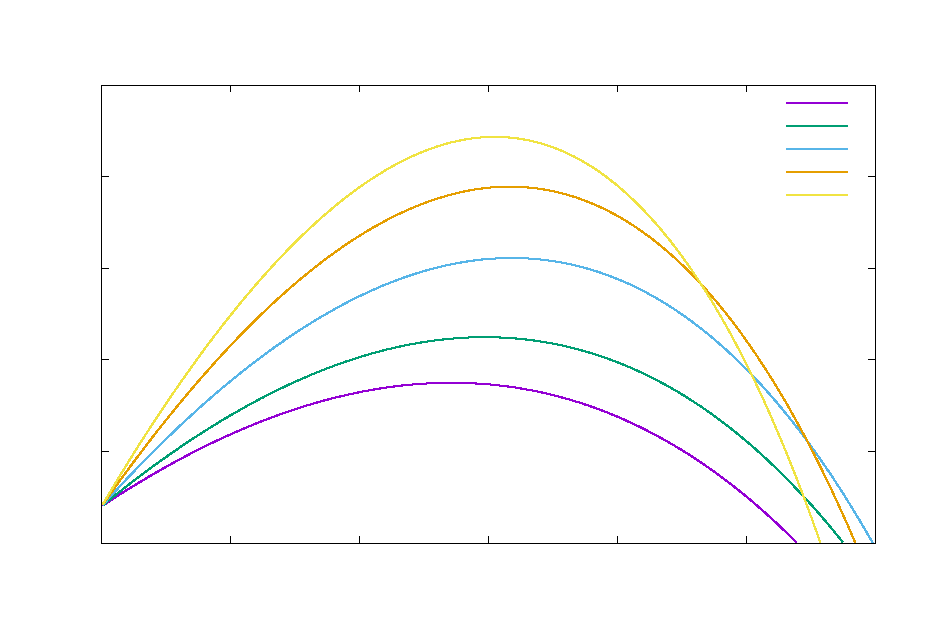
\includegraphics[width={432.00bp},height={288.00bp}]{EulerTrajectoryTEX}}%
    \gplfronttext
  \end{picture}%
\endgroup

    \caption{Figure shows trajectories of javelin thrown with different launch angles, computed using the Euler method}
    \label{fig:my_label1}
\end{figure}
\begin{itemize}
    \item We see that the ascending order of the range follows the order: 25, 50, 30, 45, 38. Therefore, we see that $x_{max}$ first increases and then decreases, peaking for 38$^\circ$.
    \item Moreover, the $y$ coordinate of the trajectory does not start from $y = 0$, since there is some height at which the javelin is released. This paper\,\cite{ref10} shows that average height stands at 1.86 m. Taking into the extension of the hand, it can be approximated to 2 m.
\end{itemize}
\newpage
\begin{figure}[H]
    \centering
    \scalebox{0.85}{% GNUPLOT: LaTeX picture with Postscript
\begingroup
  % Encoding inside the plot.  In the header of your document, this encoding
  % should to defined, e.g., by using
  % \usepackage[cp1252,<other encodings>]{inputenc}
  \inputencoding{cp1252}%
  \makeatletter
  \providecommand\color[2][]{%
    \GenericError{(gnuplot) \space\space\space\@spaces}{%
      Package color not loaded in conjunction with
      terminal option `colourtext'%
    }{See the gnuplot documentation for explanation.%
    }{Either use 'blacktext' in gnuplot or load the package
      color.sty in LaTeX.}%
    \renewcommand\color[2][]{}%
  }%
  \providecommand\includegraphics[2][]{%
    \GenericError{(gnuplot) \space\space\space\@spaces}{%
      Package graphicx or graphics not loaded%
    }{See the gnuplot documentation for explanation.%
    }{The gnuplot epslatex terminal needs graphicx.sty or graphics.sty.}%
    \renewcommand\includegraphics[2][]{}%
  }%
  \providecommand\rotatebox[2]{#2}%
  \@ifundefined{ifGPcolor}{%
    \newif\ifGPcolor
    \GPcolortrue
  }{}%
  \@ifundefined{ifGPblacktext}{%
    \newif\ifGPblacktext
    \GPblacktextfalse
  }{}%
  % define a \g@addto@macro without @ in the name:
  \let\gplgaddtomacro\g@addto@macro
  % define empty templates for all commands taking text:
  \gdef\gplbacktext{}%
  \gdef\gplfronttext{}%
  \makeatother
  \ifGPblacktext
    % no textcolor at all
    \def\colorrgb#1{}%
    \def\colorgray#1{}%
  \else
    % gray or color?
    \ifGPcolor
      \def\colorrgb#1{\color[rgb]{#1}}%
      \def\colorgray#1{\color[gray]{#1}}%
      \expandafter\def\csname LTw\endcsname{\color{white}}%
      \expandafter\def\csname LTb\endcsname{\color{black}}%
      \expandafter\def\csname LTa\endcsname{\color{black}}%
      \expandafter\def\csname LT0\endcsname{\color[rgb]{1,0,0}}%
      \expandafter\def\csname LT1\endcsname{\color[rgb]{0,1,0}}%
      \expandafter\def\csname LT2\endcsname{\color[rgb]{0,0,1}}%
      \expandafter\def\csname LT3\endcsname{\color[rgb]{1,0,1}}%
      \expandafter\def\csname LT4\endcsname{\color[rgb]{0,1,1}}%
      \expandafter\def\csname LT5\endcsname{\color[rgb]{1,1,0}}%
      \expandafter\def\csname LT6\endcsname{\color[rgb]{0,0,0}}%
      \expandafter\def\csname LT7\endcsname{\color[rgb]{1,0.3,0}}%
      \expandafter\def\csname LT8\endcsname{\color[rgb]{0.5,0.5,0.5}}%
    \else
      % gray
      \def\colorrgb#1{\color{black}}%
      \def\colorgray#1{\color[gray]{#1}}%
      \expandafter\def\csname LTw\endcsname{\color{white}}%
      \expandafter\def\csname LTb\endcsname{\color{black}}%
      \expandafter\def\csname LTa\endcsname{\color{black}}%
      \expandafter\def\csname LT0\endcsname{\color{black}}%
      \expandafter\def\csname LT1\endcsname{\color{black}}%
      \expandafter\def\csname LT2\endcsname{\color{black}}%
      \expandafter\def\csname LT3\endcsname{\color{black}}%
      \expandafter\def\csname LT4\endcsname{\color{black}}%
      \expandafter\def\csname LT5\endcsname{\color{black}}%
      \expandafter\def\csname LT6\endcsname{\color{black}}%
      \expandafter\def\csname LT7\endcsname{\color{black}}%
      \expandafter\def\csname LT8\endcsname{\color{black}}%
    \fi
  \fi
    \setlength{\unitlength}{0.0500bp}%
    \ifx\gptboxheight\undefined%
      \newlength{\gptboxheight}%
      \newlength{\gptboxwidth}%
      \newsavebox{\gptboxtext}%
    \fi%
    \setlength{\fboxrule}{0.5pt}%
    \setlength{\fboxsep}{1pt}%
    \definecolor{tbcol}{rgb}{1,1,1}%
\begin{picture}(8640.00,5760.00)%
    \gplgaddtomacro\gplbacktext{%
      \csname LTb\endcsname%%
      \put(1078,704){\makebox(0,0)[r]{\strut{}0}}%
      \put(1078,3620){\makebox(0,0)[r]{\strut{}59.72}}%
      \put(1078,4994){\makebox(0,0)[r]{\strut{}87.86}}%
      \put(1210,484){\makebox(0,0){\strut{}0$^\circ$}}%
      \put(4179,484){\makebox(0,0){\strut{}38$^\circ$}}%
      \put(4727,484){\makebox(0,0){\strut{}45$^\circ$}}%
      \put(8243,484){\makebox(0,0){\strut{}90$^\circ$}}%
    }%
    \gplgaddtomacro\gplfronttext{%
      \csname LTb\endcsname%%
      \put(209,2901){\rotatebox{-270}{\makebox(0,0){\strut{}$x_{max}$ (m)}}}%
      \put(4726,154){\makebox(0,0){\strut{}$\theta (^\circ)$}}%
      \csname LTb\endcsname%%
      \put(7256,4926){\makebox(0,0)[r]{\strut{}Without drag}}%
      \csname LTb\endcsname%%
      \put(7256,4706){\makebox(0,0)[r]{\strut{}With drag}}%
      \csname LTb\endcsname%%
      \put(4726,5429){\makebox(0,0){\strut{}RK2: Variation of $x_{max}$ with $\theta$}}%
    }%
    \gplbacktext
    \put(0,0){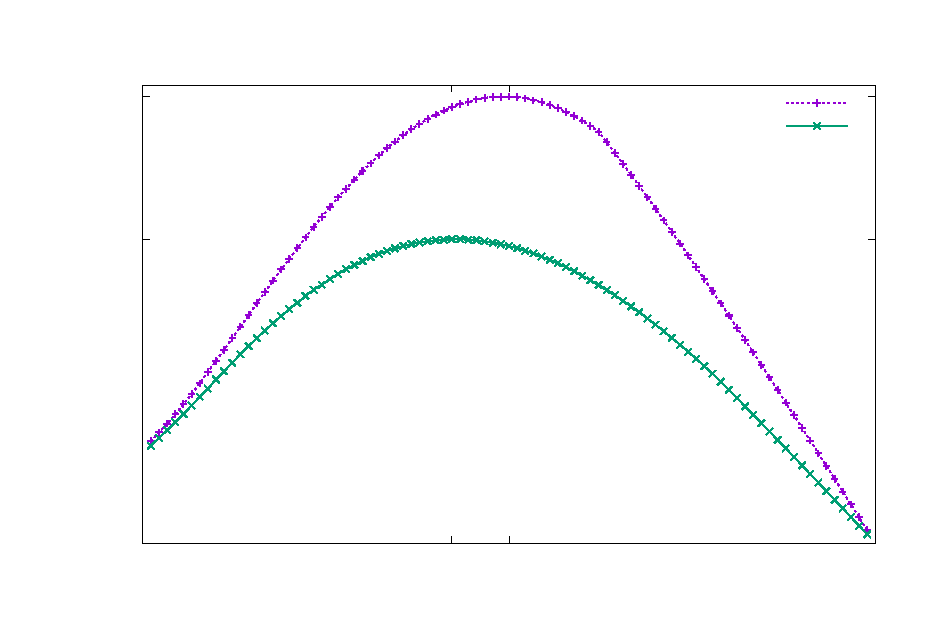
\includegraphics[width={432.00bp},height={288.00bp}]{rk2VariationTEX}}%
    \gplfronttext
  \end{picture}%
\endgroup
}
    \caption{Figure shows the variation of $x_{max}$ with $\theta$, computed using the rk2 method}
    \label{fig:my_label3}
\end{figure}
\begin{figure}[H]
    \centering
    \scalebox{0.85}{% GNUPLOT: LaTeX picture with Postscript
\begingroup
  % Encoding inside the plot.  In the header of your document, this encoding
  % should to defined, e.g., by using
  % \usepackage[cp1252,<other encodings>]{inputenc}
  \inputencoding{cp1252}%
  \makeatletter
  \providecommand\color[2][]{%
    \GenericError{(gnuplot) \space\space\space\@spaces}{%
      Package color not loaded in conjunction with
      terminal option `colourtext'%
    }{See the gnuplot documentation for explanation.%
    }{Either use 'blacktext' in gnuplot or load the package
      color.sty in LaTeX.}%
    \renewcommand\color[2][]{}%
  }%
  \providecommand\includegraphics[2][]{%
    \GenericError{(gnuplot) \space\space\space\@spaces}{%
      Package graphicx or graphics not loaded%
    }{See the gnuplot documentation for explanation.%
    }{The gnuplot epslatex terminal needs graphicx.sty or graphics.sty.}%
    \renewcommand\includegraphics[2][]{}%
  }%
  \providecommand\rotatebox[2]{#2}%
  \@ifundefined{ifGPcolor}{%
    \newif\ifGPcolor
    \GPcolortrue
  }{}%
  \@ifundefined{ifGPblacktext}{%
    \newif\ifGPblacktext
    \GPblacktextfalse
  }{}%
  % define a \g@addto@macro without @ in the name:
  \let\gplgaddtomacro\g@addto@macro
  % define empty templates for all commands taking text:
  \gdef\gplbacktext{}%
  \gdef\gplfronttext{}%
  \makeatother
  \ifGPblacktext
    % no textcolor at all
    \def\colorrgb#1{}%
    \def\colorgray#1{}%
  \else
    % gray or color?
    \ifGPcolor
      \def\colorrgb#1{\color[rgb]{#1}}%
      \def\colorgray#1{\color[gray]{#1}}%
      \expandafter\def\csname LTw\endcsname{\color{white}}%
      \expandafter\def\csname LTb\endcsname{\color{black}}%
      \expandafter\def\csname LTa\endcsname{\color{black}}%
      \expandafter\def\csname LT0\endcsname{\color[rgb]{1,0,0}}%
      \expandafter\def\csname LT1\endcsname{\color[rgb]{0,1,0}}%
      \expandafter\def\csname LT2\endcsname{\color[rgb]{0,0,1}}%
      \expandafter\def\csname LT3\endcsname{\color[rgb]{1,0,1}}%
      \expandafter\def\csname LT4\endcsname{\color[rgb]{0,1,1}}%
      \expandafter\def\csname LT5\endcsname{\color[rgb]{1,1,0}}%
      \expandafter\def\csname LT6\endcsname{\color[rgb]{0,0,0}}%
      \expandafter\def\csname LT7\endcsname{\color[rgb]{1,0.3,0}}%
      \expandafter\def\csname LT8\endcsname{\color[rgb]{0.5,0.5,0.5}}%
    \else
      % gray
      \def\colorrgb#1{\color{black}}%
      \def\colorgray#1{\color[gray]{#1}}%
      \expandafter\def\csname LTw\endcsname{\color{white}}%
      \expandafter\def\csname LTb\endcsname{\color{black}}%
      \expandafter\def\csname LTa\endcsname{\color{black}}%
      \expandafter\def\csname LT0\endcsname{\color{black}}%
      \expandafter\def\csname LT1\endcsname{\color{black}}%
      \expandafter\def\csname LT2\endcsname{\color{black}}%
      \expandafter\def\csname LT3\endcsname{\color{black}}%
      \expandafter\def\csname LT4\endcsname{\color{black}}%
      \expandafter\def\csname LT5\endcsname{\color{black}}%
      \expandafter\def\csname LT6\endcsname{\color{black}}%
      \expandafter\def\csname LT7\endcsname{\color{black}}%
      \expandafter\def\csname LT8\endcsname{\color{black}}%
    \fi
  \fi
    \setlength{\unitlength}{0.0500bp}%
    \ifx\gptboxheight\undefined%
      \newlength{\gptboxheight}%
      \newlength{\gptboxwidth}%
      \newsavebox{\gptboxtext}%
    \fi%
    \setlength{\fboxrule}{0.5pt}%
    \setlength{\fboxsep}{1pt}%
    \definecolor{tbcol}{rgb}{1,1,1}%
\begin{picture}(8640.00,5760.00)%
    \gplgaddtomacro\gplbacktext{%
      \csname LTb\endcsname%%
      \put(682,704){\makebox(0,0)[r]{\strut{}$0$}}%
      \put(682,1583){\makebox(0,0)[r]{\strut{}$5$}}%
      \put(682,2462){\makebox(0,0)[r]{\strut{}$10$}}%
      \put(682,3341){\makebox(0,0)[r]{\strut{}$15$}}%
      \put(682,4220){\makebox(0,0)[r]{\strut{}$20$}}%
      \put(682,5099){\makebox(0,0)[r]{\strut{}$25$}}%
      \put(814,484){\makebox(0,0){\strut{}$0$}}%
      \put(2052,484){\makebox(0,0){\strut{}$10$}}%
      \put(3290,484){\makebox(0,0){\strut{}$20$}}%
      \put(4529,484){\makebox(0,0){\strut{}$30$}}%
      \put(5767,484){\makebox(0,0){\strut{}$40$}}%
      \put(7005,484){\makebox(0,0){\strut{}$50$}}%
      \put(8243,484){\makebox(0,0){\strut{}$60$}}%
    }%
    \gplgaddtomacro\gplfronttext{%
      \csname LTb\endcsname%%
      \put(209,2901){\rotatebox{-270}{\makebox(0,0){\strut{}$y$ m}}}%
      \put(4528,154){\makebox(0,0){\strut{}$x$ m}}%
      \csname LTb\endcsname%%
      \put(7256,4926){\makebox(0,0)[r]{\strut{}25$^\circ$}}%
      \csname LTb\endcsname%%
      \put(7256,4706){\makebox(0,0)[r]{\strut{}30$^\circ$}}%
      \csname LTb\endcsname%%
      \put(7256,4486){\makebox(0,0)[r]{\strut{}38$^\circ$}}%
      \csname LTb\endcsname%%
      \put(7256,4266){\makebox(0,0)[r]{\strut{}45$^\circ$}}%
      \csname LTb\endcsname%%
      \put(7256,4046){\makebox(0,0)[r]{\strut{}50$^\circ$}}%
      \csname LTb\endcsname%%
      \put(4528,5429){\makebox(0,0){\strut{}RK2: Trajectory of various different launch angles, with drag}}%
    }%
    \gplbacktext
    \put(0,0){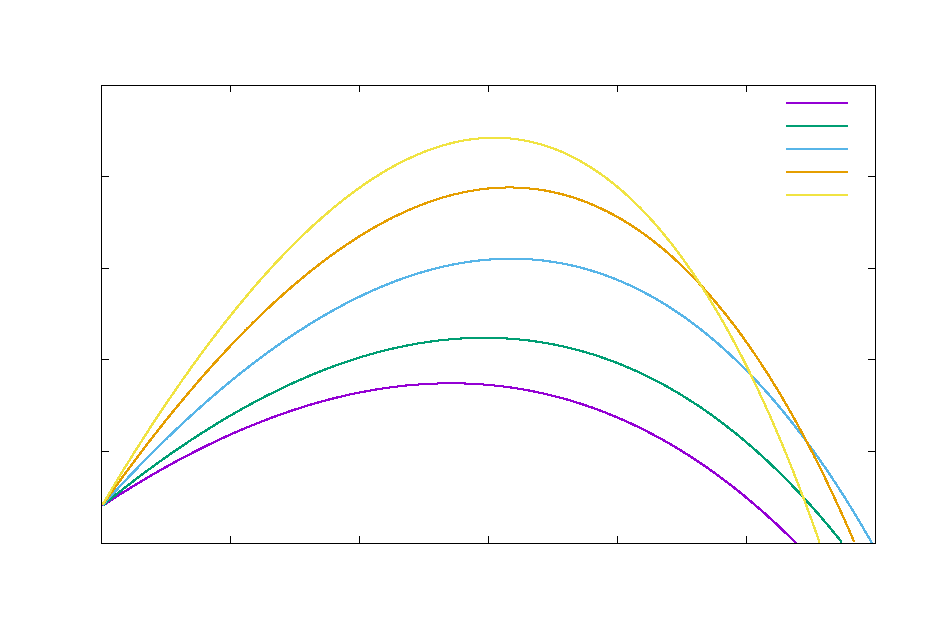
\includegraphics[width={432.00bp},height={288.00bp}]{rk2TrajectoryTEX}}%
    \gplfronttext
  \end{picture}%
\endgroup
}
    \caption{Figure shows trajectories of javelin thrown with different launch angles, computed using the rk2 method}
    \label{fig:my_label4}
\end{figure}
\begin{figure}[H]
    \centering
    \scalebox{0.85}{% GNUPLOT: LaTeX picture with Postscript
\begingroup
  % Encoding inside the plot.  In the header of your document, this encoding
  % should to defined, e.g., by using
  % \usepackage[cp1252,<other encodings>]{inputenc}
  \inputencoding{cp1252}%
  \makeatletter
  \providecommand\color[2][]{%
    \GenericError{(gnuplot) \space\space\space\@spaces}{%
      Package color not loaded in conjunction with
      terminal option `colourtext'%
    }{See the gnuplot documentation for explanation.%
    }{Either use 'blacktext' in gnuplot or load the package
      color.sty in LaTeX.}%
    \renewcommand\color[2][]{}%
  }%
  \providecommand\includegraphics[2][]{%
    \GenericError{(gnuplot) \space\space\space\@spaces}{%
      Package graphicx or graphics not loaded%
    }{See the gnuplot documentation for explanation.%
    }{The gnuplot epslatex terminal needs graphicx.sty or graphics.sty.}%
    \renewcommand\includegraphics[2][]{}%
  }%
  \providecommand\rotatebox[2]{#2}%
  \@ifundefined{ifGPcolor}{%
    \newif\ifGPcolor
    \GPcolortrue
  }{}%
  \@ifundefined{ifGPblacktext}{%
    \newif\ifGPblacktext
    \GPblacktextfalse
  }{}%
  % define a \g@addto@macro without @ in the name:
  \let\gplgaddtomacro\g@addto@macro
  % define empty templates for all commands taking text:
  \gdef\gplbacktext{}%
  \gdef\gplfronttext{}%
  \makeatother
  \ifGPblacktext
    % no textcolor at all
    \def\colorrgb#1{}%
    \def\colorgray#1{}%
  \else
    % gray or color?
    \ifGPcolor
      \def\colorrgb#1{\color[rgb]{#1}}%
      \def\colorgray#1{\color[gray]{#1}}%
      \expandafter\def\csname LTw\endcsname{\color{white}}%
      \expandafter\def\csname LTb\endcsname{\color{black}}%
      \expandafter\def\csname LTa\endcsname{\color{black}}%
      \expandafter\def\csname LT0\endcsname{\color[rgb]{1,0,0}}%
      \expandafter\def\csname LT1\endcsname{\color[rgb]{0,1,0}}%
      \expandafter\def\csname LT2\endcsname{\color[rgb]{0,0,1}}%
      \expandafter\def\csname LT3\endcsname{\color[rgb]{1,0,1}}%
      \expandafter\def\csname LT4\endcsname{\color[rgb]{0,1,1}}%
      \expandafter\def\csname LT5\endcsname{\color[rgb]{1,1,0}}%
      \expandafter\def\csname LT6\endcsname{\color[rgb]{0,0,0}}%
      \expandafter\def\csname LT7\endcsname{\color[rgb]{1,0.3,0}}%
      \expandafter\def\csname LT8\endcsname{\color[rgb]{0.5,0.5,0.5}}%
    \else
      % gray
      \def\colorrgb#1{\color{black}}%
      \def\colorgray#1{\color[gray]{#1}}%
      \expandafter\def\csname LTw\endcsname{\color{white}}%
      \expandafter\def\csname LTb\endcsname{\color{black}}%
      \expandafter\def\csname LTa\endcsname{\color{black}}%
      \expandafter\def\csname LT0\endcsname{\color{black}}%
      \expandafter\def\csname LT1\endcsname{\color{black}}%
      \expandafter\def\csname LT2\endcsname{\color{black}}%
      \expandafter\def\csname LT3\endcsname{\color{black}}%
      \expandafter\def\csname LT4\endcsname{\color{black}}%
      \expandafter\def\csname LT5\endcsname{\color{black}}%
      \expandafter\def\csname LT6\endcsname{\color{black}}%
      \expandafter\def\csname LT7\endcsname{\color{black}}%
      \expandafter\def\csname LT8\endcsname{\color{black}}%
    \fi
  \fi
    \setlength{\unitlength}{0.0500bp}%
    \ifx\gptboxheight\undefined%
      \newlength{\gptboxheight}%
      \newlength{\gptboxwidth}%
      \newsavebox{\gptboxtext}%
    \fi%
    \setlength{\fboxrule}{0.5pt}%
    \setlength{\fboxsep}{1pt}%
    \definecolor{tbcol}{rgb}{1,1,1}%
\begin{picture}(8640.00,5760.00)%
    \gplgaddtomacro\gplbacktext{%
      \csname LTb\endcsname%%
      \put(1078,704){\makebox(0,0)[r]{\strut{}0}}%
      \put(1078,3620){\makebox(0,0)[r]{\strut{}59.72}}%
      \put(1078,4994){\makebox(0,0)[r]{\strut{}87.86}}%
      \put(1210,484){\makebox(0,0){\strut{}0$^\circ$}}%
      \put(4179,484){\makebox(0,0){\strut{}38$^\circ$}}%
      \put(4727,484){\makebox(0,0){\strut{}45$^\circ$}}%
      \put(8243,484){\makebox(0,0){\strut{}90$^\circ$}}%
    }%
    \gplgaddtomacro\gplfronttext{%
      \csname LTb\endcsname%%
      \put(209,2901){\rotatebox{-270}{\makebox(0,0){\strut{}$x_{max}$ (m)}}}%
      \put(4726,154){\makebox(0,0){\strut{}$\theta (^\circ)$}}%
      \csname LTb\endcsname%%
      \put(7256,4926){\makebox(0,0)[r]{\strut{}Without drag}}%
      \csname LTb\endcsname%%
      \put(7256,4706){\makebox(0,0)[r]{\strut{}With drag}}%
      \csname LTb\endcsname%%
      \put(4726,5429){\makebox(0,0){\strut{}RK4: Variation of $x_{max}$ with $\theta$}}%
    }%
    \gplbacktext
    \put(0,0){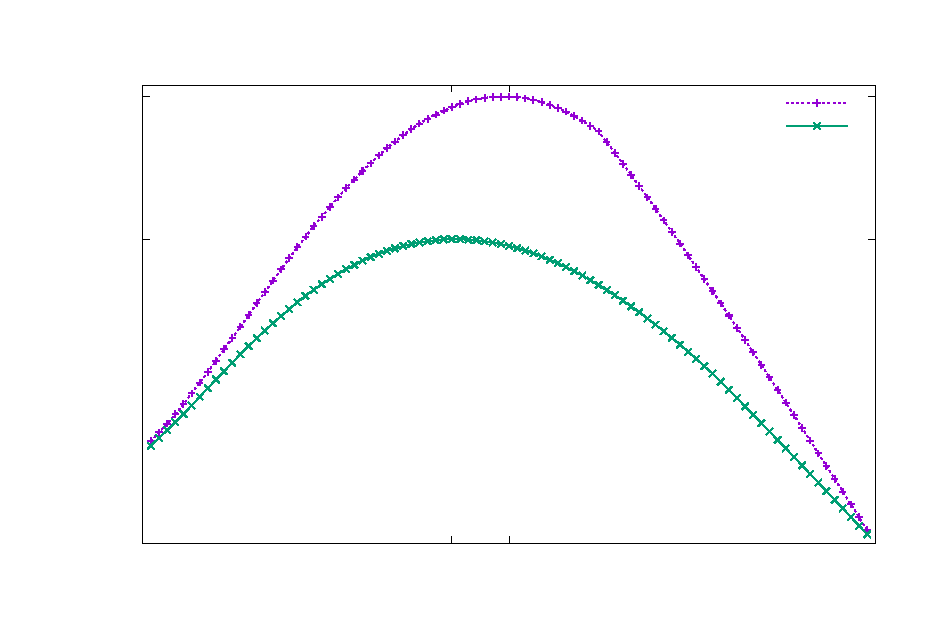
\includegraphics[width={432.00bp},height={288.00bp}]{rk4VariationTEX}}%
    \gplfronttext
  \end{picture}%
\endgroup
}
    \caption{Figure shows the variation of $x_{max}$ with $\theta$, computed using the rk4 method}
    \label{fig:my_label5}
\end{figure}
\begin{figure}[H]
    \centering
    \scalebox{0.85}{% GNUPLOT: LaTeX picture with Postscript
\begingroup
  % Encoding inside the plot.  In the header of your document, this encoding
  % should to defined, e.g., by using
  % \usepackage[cp1252,<other encodings>]{inputenc}
  \inputencoding{cp1252}%
  \makeatletter
  \providecommand\color[2][]{%
    \GenericError{(gnuplot) \space\space\space\@spaces}{%
      Package color not loaded in conjunction with
      terminal option `colourtext'%
    }{See the gnuplot documentation for explanation.%
    }{Either use 'blacktext' in gnuplot or load the package
      color.sty in LaTeX.}%
    \renewcommand\color[2][]{}%
  }%
  \providecommand\includegraphics[2][]{%
    \GenericError{(gnuplot) \space\space\space\@spaces}{%
      Package graphicx or graphics not loaded%
    }{See the gnuplot documentation for explanation.%
    }{The gnuplot epslatex terminal needs graphicx.sty or graphics.sty.}%
    \renewcommand\includegraphics[2][]{}%
  }%
  \providecommand\rotatebox[2]{#2}%
  \@ifundefined{ifGPcolor}{%
    \newif\ifGPcolor
    \GPcolortrue
  }{}%
  \@ifundefined{ifGPblacktext}{%
    \newif\ifGPblacktext
    \GPblacktextfalse
  }{}%
  % define a \g@addto@macro without @ in the name:
  \let\gplgaddtomacro\g@addto@macro
  % define empty templates for all commands taking text:
  \gdef\gplbacktext{}%
  \gdef\gplfronttext{}%
  \makeatother
  \ifGPblacktext
    % no textcolor at all
    \def\colorrgb#1{}%
    \def\colorgray#1{}%
  \else
    % gray or color?
    \ifGPcolor
      \def\colorrgb#1{\color[rgb]{#1}}%
      \def\colorgray#1{\color[gray]{#1}}%
      \expandafter\def\csname LTw\endcsname{\color{white}}%
      \expandafter\def\csname LTb\endcsname{\color{black}}%
      \expandafter\def\csname LTa\endcsname{\color{black}}%
      \expandafter\def\csname LT0\endcsname{\color[rgb]{1,0,0}}%
      \expandafter\def\csname LT1\endcsname{\color[rgb]{0,1,0}}%
      \expandafter\def\csname LT2\endcsname{\color[rgb]{0,0,1}}%
      \expandafter\def\csname LT3\endcsname{\color[rgb]{1,0,1}}%
      \expandafter\def\csname LT4\endcsname{\color[rgb]{0,1,1}}%
      \expandafter\def\csname LT5\endcsname{\color[rgb]{1,1,0}}%
      \expandafter\def\csname LT6\endcsname{\color[rgb]{0,0,0}}%
      \expandafter\def\csname LT7\endcsname{\color[rgb]{1,0.3,0}}%
      \expandafter\def\csname LT8\endcsname{\color[rgb]{0.5,0.5,0.5}}%
    \else
      % gray
      \def\colorrgb#1{\color{black}}%
      \def\colorgray#1{\color[gray]{#1}}%
      \expandafter\def\csname LTw\endcsname{\color{white}}%
      \expandafter\def\csname LTb\endcsname{\color{black}}%
      \expandafter\def\csname LTa\endcsname{\color{black}}%
      \expandafter\def\csname LT0\endcsname{\color{black}}%
      \expandafter\def\csname LT1\endcsname{\color{black}}%
      \expandafter\def\csname LT2\endcsname{\color{black}}%
      \expandafter\def\csname LT3\endcsname{\color{black}}%
      \expandafter\def\csname LT4\endcsname{\color{black}}%
      \expandafter\def\csname LT5\endcsname{\color{black}}%
      \expandafter\def\csname LT6\endcsname{\color{black}}%
      \expandafter\def\csname LT7\endcsname{\color{black}}%
      \expandafter\def\csname LT8\endcsname{\color{black}}%
    \fi
  \fi
    \setlength{\unitlength}{0.0500bp}%
    \ifx\gptboxheight\undefined%
      \newlength{\gptboxheight}%
      \newlength{\gptboxwidth}%
      \newsavebox{\gptboxtext}%
    \fi%
    \setlength{\fboxrule}{0.5pt}%
    \setlength{\fboxsep}{1pt}%
    \definecolor{tbcol}{rgb}{1,1,1}%
\begin{picture}(8640.00,5760.00)%
    \gplgaddtomacro\gplbacktext{%
      \csname LTb\endcsname%%
      \put(682,704){\makebox(0,0)[r]{\strut{}$0$}}%
      \put(682,1583){\makebox(0,0)[r]{\strut{}$5$}}%
      \put(682,2462){\makebox(0,0)[r]{\strut{}$10$}}%
      \put(682,3341){\makebox(0,0)[r]{\strut{}$15$}}%
      \put(682,4220){\makebox(0,0)[r]{\strut{}$20$}}%
      \put(682,5099){\makebox(0,0)[r]{\strut{}$25$}}%
      \put(814,484){\makebox(0,0){\strut{}$0$}}%
      \put(2052,484){\makebox(0,0){\strut{}$10$}}%
      \put(3290,484){\makebox(0,0){\strut{}$20$}}%
      \put(4529,484){\makebox(0,0){\strut{}$30$}}%
      \put(5767,484){\makebox(0,0){\strut{}$40$}}%
      \put(7005,484){\makebox(0,0){\strut{}$50$}}%
      \put(8243,484){\makebox(0,0){\strut{}$60$}}%
    }%
    \gplgaddtomacro\gplfronttext{%
      \csname LTb\endcsname%%
      \put(209,2901){\rotatebox{-270}{\makebox(0,0){\strut{}$y$ m}}}%
      \put(4528,154){\makebox(0,0){\strut{}$x$ m}}%
      \csname LTb\endcsname%%
      \put(7256,4926){\makebox(0,0)[r]{\strut{}25$^\circ$}}%
      \csname LTb\endcsname%%
      \put(7256,4706){\makebox(0,0)[r]{\strut{}30$^\circ$}}%
      \csname LTb\endcsname%%
      \put(7256,4486){\makebox(0,0)[r]{\strut{}38$^\circ$}}%
      \csname LTb\endcsname%%
      \put(7256,4266){\makebox(0,0)[r]{\strut{}45$^\circ$}}%
      \csname LTb\endcsname%%
      \put(7256,4046){\makebox(0,0)[r]{\strut{}50$^\circ$}}%
      \csname LTb\endcsname%%
      \put(4528,5429){\makebox(0,0){\strut{}RK4: Trajectory of various different launch angles, with drag}}%
    }%
    \gplbacktext
    \put(0,0){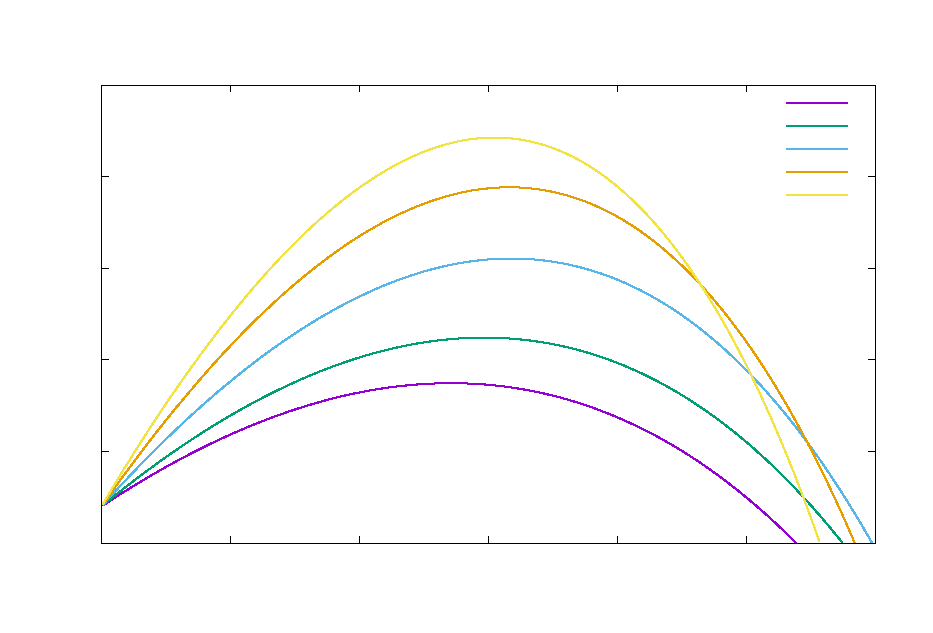
\includegraphics[width={432.00bp},height={288.00bp}]{rk4TrajectoryTEX}}%
    \gplfronttext
  \end{picture}%
\endgroup
}
    \caption{Figure shows trajectories of javelin thrown with different launch angles, computed using the rk4 method}
    \label{fig:my_label6}
\end{figure}
\newpage
In the last two pages, shown are the figures whose data is computed using the rk2, and rk4 methods. Based on the plots, we make the following assertions, and reasons:
\begin{itemize}
    \item The results by and large remain the same, and so do the conclusions, since the angle for maximization of the range still comes out to be 38$^\circ$.
    \item However, due to a difference in algorithm the computed value of $x_{max}$ changes from 59.8m to 59.72m. 
    \item The difference stated above could've been reduced by increasing the number of divisions, and or decreasing the step-size. However, computational physics has its own limits in terms of computing power.
\end{itemize}
\newpage
%%%%%%%%%%%%%%%%%%%%%%%%%%%%%%%%%%%%%%
\section{Summary}
\label{sec:summary}
Evolving from our common love of sports and physics, the primary objective of this project was to study a object in projectile motion taking air drag into account and see if could come up an angle of release that is more realistic that what we are usually taught, in order to maximize the horizontal range of the object under projectile motion. One of the key findings of our project was as we take the friction into account as the viscous force of air, acting against the direction of motion, we optimum angle of release to maximize the horizontal range came out to be 38$^\circ$ with all the three methods. This helps to put things in perspective taking friction into account, as friction is always an uncharted territory in physics. Exploration of this territory results in some more realistic answers, which might help athletes mend their training and throwing styles for good. Moreover, it helps the students understand how to take the friction into account, since if there is one phrase which happens to be around more than others is \textit{ignore friction}, or \textit{neglect air} resistance. Now there are, as one might expect with a project involving a pinch of aerodynamics and estimation of frictional forces, some limitations of the project. First are the methods that we have used to solve our simultaneous differential equations themselves. \\
First, of all, all these methods provide an approximate solution to the differential equation and not exact. Moreover, numerical methods to solve differential equations are often very lengthy and are solved using computers, and to get fairly accurate results, they sometimes may require high computational power. This basically means that the more accurate you want your results to be, the more number of iterations your computer should be able to do, and therefore, higher should be its computational power.\\
Next comes the value of the coefficient of friction. Many assumptions were made in this section, that might not always happen. Taking the speed of wind to be zero, so that we can estimate the relative velocity of wind and the javelin solely on the basis of the velocity of the former, is one. However, the future scope of this research is quite open. Sport organisations may collect empirical data to conduct a similar research instead of using numerical methods. In this way, they will overcome both of our limitations, that is the limited reliability of numerical methods and the estimation of coefficient of friction. The fact that this research would have athletes optimize their performance in a major Olympics sport, that is javelin throw, shows the commercial viability of such research in future. 
\newpage
%%%%%%%%%%%%%%%%%%%%%%%%%%%%%%
\begin{thebibliography}{}
\bibitem{ref1}
\href{https://indianexpress.com/article/olympics/elasticity-perfect-angle-speed-what-worked-for-neeraj-chopra-7443674/}{Koshie, N (2021, August 8). Elasticity, perfect angle, speed: What worked for Neeraj Chopra. \textit{The Indian Express}}
\bibitem{ref5}
Landau, R.H., Paez, M.J., and Bordeianu, C.C., (2007). \textit{Computational Physics} WILEY-VCH Verlag GmbH and Co. KGaA, Weinheim
\bibitem{ref2}
\href{https://ncert.nic.in/textbook/pdf/keph104.pdf}{N.C.E.R.T. (2010), \textit{Physics Part I - Textbook for class XI}, Publication Department, National Council of Educational Research and Training}
\bibitem{ref3}
\href{https://ncert.nic.in/textbook/pdf/keph104.pdf}{N.C.E.R.T. (2010), \textit{Physics Part I - Textbook for class XI}, Publication Department, National Council of Educational Research and Training}
\bibitem{ref11}
\href{https://theconversation.com/science-of-the-spear-biomechanics-of-a-javelin-throw-29782}{Barber, M. (July 31, 2014), \textit{Science of the spear: biomechanics of a javelin throw}. Retrieved Nov 10, 2021}
\bibitem{ref12}
\href{https://theconversation.com/science-of-the-spear-biomechanics-of-a-javelin-throw-29782}{Barber, M. (July 31, 2014), \textit{Science of the spear: biomechanics of a javelin throw}. Retrieved Nov 10, 2021}
\bibitem{ref4}
\href{https://www.sportsrec.com/6929852/physics-of-javelin-throwing}{Brooker, J (November 16, 2018): \textit{Physics of Javelin throwing}. Retrieved Nov 7, 2021.}
\bibitem{ref6}
\href{https://arc.aiaa.org/doi/abs/10.2514/6.2021-1871}{Okuizumi, H., Sasaki, K., Konishi, Y., and Obayashi, S. (2021). Aerodynamic Characteristics of Javelin Measured with 1-m Magnetic Suspension and Balance System. In AIAA Scitech 2021 Forum (p. 1871).}
\bibitem{ref7}
\href{https://www.engineeringtoolbox.com/air-density-specific-weight-d_600.html}{N.A. (n.d.) \textit{Air - Density, Specific Weight and Thermal expansion coefficient vs Temperature and Pressure} Retrieved November 7, 2021}
\bibitem{ref8}
\href{https://www.sportsunlimitedinc.com/sportsu-javelin.html}{N.A. (n.d.) \textit{Javelin Throw Guide.} Retrieved November 7, 2021}
\bibitem{ref9}
\href{https://www.sportsunlimitedinc.com/sportsu-javelin.html}{N.A. (n.d.) \textit{Javelin Throw Guide.} Retrieved November 7, 2021}
\bibitem{ref10}
\href{https://ojs.ub.uni-konstanz.de/cpa/article/view/3783}{Coh, M., Embersic, D., \& Zvan, M. (2001). Correlation between anthropometric characteristics and competitive results of elite junior javelin throwers.}
\end{thebibliography}

%%%%%%%%%%%%%%%%%%%%%%%%%%%%%%%
\newpage 
\appendix
\section{Programs}
Python program
\begin{lstlisting}[language=Python, caption=Python code]
import numpy as np
import math
import pandas as pd

def f(t, Y0, Y1, Y2, Y3, case):
  if case == "drag":
    k = 0.5*1.255*2.5*0.003
  else: 
    k = 0
  fx_drag = -1*k*29*Y1
  fy_drag = -1*k*29*Y3
  m = 0.8
  fni_Y0 = Y1
  fni_Y1 = fx_drag/m
  fni_Y2 = Y3
  fni_Y3 = fy_drag/m - 9.8
  return fni_Y0, fni_Y1, fni_Y2, fni_Y3

def euler(Y0, Y1, Y2, Y3, a, b, case, l1, grph_key, file_name): 
  N = 1000
  h = (b - a)/N
  tn = []
  Y0n = []
  Y1n = []
  Y2n = []
  Y3n = []
  for i in range(0, N):
    t = a + i*h
    tn.append(t)
    Y0n.append(Y0)
    Y1n.append(Y1)
    Y2n.append(Y2)
    Y3n.append(Y3)
    fni_Y0, fni_Y1, fni_Y2, fni_Y3 = f(t, Y0, Y1, Y2, Y3, case)
    Y0 = Y0 + h*fni_Y0
    Y1 = Y1 + h*fni_Y1
    Y2 = Y2 + h*fni_Y2
    Y3 = Y3 + h*fni_Y3
    if Y2<=0:
      break   
  if grph_key == 0:
    if case == "no drag":
      print()
    else:
      data_euler_1 = {"x": Y0n, "y" : Y2n}
      my_data111 = pd.DataFrame(data_euler_1)
      my_data111.to_csv(file_name, index = False)
  else:
    return Y0n[-1]

def rk4(Y0, Y1, Y2, Y3, a, b, case, l1, grph_key, file_name): 
  N = 1000
  h = (b - a)/N
  tn = []
  Y0n = []
  Y1n = []
  Y2n = []
  Y3n = []
  for i in range(0, N):
    t = a + i*h
    tn.append(t)
    Y0n.append(Y0)
    Y1n.append(Y1)
    Y2n.append(Y2)
    Y3n.append(Y3)
    m1_0, m1_1, m1_2, m1_3 = f(t, Y0, Y1, Y2, Y3, case)
    m2_0, m2_1, m2_2, m2_3 = f(t + h/2, Y0 + m1_0*h/2, Y1 + m1_1*h/2, Y2 + m1_2*h/2, Y3 + m1_3*h/2, case)
    m3_0, m3_1, m3_2, m3_3 = f(t + h/2, Y0 + m2_0*h/2, Y1 + m2_1*h/2, Y2 + m2_2*h/2, Y3 + m2_3*h/2, case)
    m4_0, m4_1, m4_2, m4_3 = f(t + h, Y0 + m3_0*h, Y1 + m3_1*h, Y2 + m3_1*h, Y3 + m3_1*h, case)
    mrk4_0 = (m1_0 + 2*m2_0 + 2*m3_0 + m4_0)/6
    mrk4_1 = (m1_1 + 2*m2_1 + 2*m3_1 + m4_1)/6
    mrk4_2 = (m1_2 + 2*m2_2 + 2*m3_2 + m4_2)/6
    mrk4_3 = (m1_3 + 2*m2_3 + 2*m3_3 + m4_3)/6
    Y0 = Y0 + h*mrk4_0
    Y1 = Y1 + h*mrk4_1
    Y2 = Y2 + h*mrk4_2
    Y3 = Y3 + h*mrk4_3
    if Y2<=0:
      break   
  if grph_key == 0:
    if case == "no drag":
      print()
    else:
      data_rk4_1 = {"x": Y0n, "y" : Y2n}
      my_data112 = pd.DataFrame(data_rk4_1)
      my_data112.to_csv(file_name, index = False)
  else:
    return Y0n[-1]

def rk2(Y0, Y1, Y2, Y3, a, b, case, l1, grph_key, file_name): 
  N = 1000
  h = (b - a)/N
  tn = []
  Y0n = []
  Y1n = []
  Y2n = []
  Y3n = []
  for i in range(0, N):
    t = a + i*h
    tn.append(t)
    Y0n.append(Y0)
    Y1n.append(Y1)
    Y2n.append(Y2)
    Y3n.append(Y3)
    k1_0, k1_1, k1_2, k1_3 = f(t, Y0, Y1, Y2, Y3, case)
    k1_0, k1_1, k1_2, k1_3 = h*k1_0, h*k1_1, h*k1_2, h*k1_3
    k2_0, k2_1, k2_2, k2_3 = f(t+h, Y0 + k1_0, Y1 + k1_1, Y2 + k1_2, Y3 + k1_3, case)
    k2_0, k2_1, k2_2, k2_3 = h*k2_0, h*k2_1, h*k2_2, h*k2_3
    Y0 = Y0 + (k1_0 + k2_0)/2
    Y1 = Y1 + (k1_1 + k2_1)/2
    Y2 = Y2 + (k1_2 + k2_2)/2
    Y3 = Y3 + (k1_3 + k2_3)/2
    if Y2<=0:
      break   
  if grph_key == 0:
    if case == "no drag":
      print()
    else:
      data_rk2_1 = {"x": Y0n, "y" : Y2n}
      my_data113 = pd.DataFrame(data_rk2_1)
      my_data113.to_csv(file_name, index = False)
  else:
    return Y0n[-1]

#CALL:
angle_list = [25, 30, 45, 50, 38]
file_names_euler =['EulerTrajectory25.csv', 'EulerTrajectory30.csv', 'EulerTrajectory45.csv', 'EulerTrajectory50.csv', 'EulerTrajectory38.csv']
file_names_rk2 =['rk2Trajectory25.csv', 'rk2Trajectory30.csv', 'rk2Trajectory45.csv', 'rk2Trajectory50.csv', 'rk2Trajectory38.csv']
file_names_rk4 =['rk4Trajectory25.csv', 'rk4Trajectory30.csv', 'rk4Trajectory45.csv', 'rk4Trajectory50.csv', 'rk4Trajectory38.csv']
label_list = ["25$^{\circ}$", "30$^{\circ}$", "45$^{\circ}$", "50$^{\circ}$", "38$^{\circ}$"]

for i in range(0, 5):
  Y3 = 29*math.sin(0.0174533*angle_list[i])
  Y1 = 29*math.cos(0.0174533*angle_list[i])
  euler(0, Y1, 2, Y3, 0, 5, "drag", label_list[i], 0, file_names_euler[i])

for i in range(0, 5):
  Y3 = 29*math.sin(0.0174533*angle_list[i])
  Y1 = 29*math.cos(0.0174533*angle_list[i])
  rk2(0, Y1, 2, Y3, 0, 5, "drag", label_list[i], 0, file_names_rk2[i])

for i in range(0, 5):
  Y3 = 29*math.sin(0.0174533*angle_list[i])
  Y1 = 29*math.cos(0.0174533*angle_list[i])
  rk4(0, Y1, 2, Y3, 0, 5, "drag", label_list[i], 0, file_names_rk4[i])

angle = []
x_with_drag_euler = []
x_without_drag_euler = []
row_euler = []
record_euler = []
x_with_drag_rk2 = []
x_without_drag_rk2 = []
row_rk2 = []
record_rk2 = []
x_with_drag_rk4 = []
x_without_drag_rk4 = []
row_rk4 = []
record_rk4 = []

for i in range(0, 90):
  Y3 = 29*math.sin(0.0174533*i)
  Y1 = 29*math.cos(0.0174533*i)
  xn_with_drag_euler = euler(0, Y1, 2, Y3, 0, 5, "drag", label_list[0], 1, 'does not matter')
  xn_without_drag_euler = euler(0, Y1, 2, Y3, 0, 5, "no drag", label_list[0], 1, 'does not matter')
  x_with_drag_euler.append(xn_with_drag_euler)
  x_without_drag_euler.append(xn_without_drag_euler)
  angle.append(i)
  row_euler.append(i)
  row_euler.append(xn_with_drag_euler)
  record_euler.append(row_euler)
  row_euler = []
data_euler_2_wo = {"theta": angle, "range" : x_without_drag_euler}
my_data211 = pd.DataFrame(data_euler_2_wo)
my_data211.to_csv('EulerVariationWO.csv', index = False)
data_euler_2_w = {"theta": angle, "range" : x_with_drag_euler}
my_data212 = pd.DataFrame(data_euler_2_w)
my_data212.to_csv('EulerVariationW.csv', index = False)

for i in range(0, 90):
  Y3 = 29*math.sin(0.0174533*i)
  Y1 = 29*math.cos(0.0174533*i)
  xn_with_drag_rk2 = rk2(0, Y1, 2, Y3, 0, 5, "drag", label_list[0], 1, 'does not matter')
  xn_without_drag_rk2 = rk2(0, Y1, 2, Y3, 0, 5, "no drag", label_list[0], 1, 'does not matter')
  x_with_drag_rk2.append(xn_with_drag_rk2)
  x_without_drag_rk2.append(xn_without_drag_rk2)
  row_rk2.append(i)
  row_rk2.append(xn_with_drag_rk2)
  record_rk2.append(row_rk2)
  row_rk2 = []
data_rk2_2_wo = {"theta": angle, "range" : x_without_drag_rk2}
my_data221 = pd.DataFrame(data_rk2_2_wo)
my_data221.to_csv('rk2VariationWO.csv', index = False)
data_rk2_2_w = {"theta": angle, "range" : x_with_drag_rk2}
my_data222 = pd.DataFrame(data_rk2_2_w)
my_data222.to_csv('rk2VariationW.csv', index = False)

for i in range(0, 90):
  Y3 = 29*math.sin(0.0174533*i)
  Y1 = 29*math.cos(0.0174533*i)
  xn_with_drag_rk4 = rk4(0, Y1, 2, Y3, 0, 5, "drag", label_list[0], 1, 'does not matter')
  xn_without_drag_rk4 = rk4(0, Y1, 2, Y3, 0, 5, "no drag", label_list[0], 1, 'does not matter')
  x_with_drag_rk4.append(xn_with_drag_rk4)
  x_without_drag_rk4.append(xn_without_drag_rk4)
  row_rk4.append(i)
  row_rk4.append(xn_with_drag_rk4)
  record_rk4.append(row_rk4)
  row_rk4 = []
data_rk4_2_wo = {"theta": angle, "range" : x_without_drag_rk4}
my_data231 = pd.DataFrame(data_rk4_2_wo)
my_data231.to_csv('rk4VariationWO.csv', index = False)
data_rk4_2_w = {"theta": angle, "range" : x_with_drag_rk4}
my_data232 = pd.DataFrame(data_rk4_2_w)
my_data232.to_csv('rk4VariationW.csv', index = False)
\end{lstlisting}
\newpage 
GNU Plot Scripts:\\
1. "Script.txt": This file calls all the other scripts, and stands as a standalone file to be loaded into GNU plot terimal to produce all the graphs
\begin{lstlisting}[language=Python, caption="Script.txt"]
load "EULER trajectory.txt"
load "RK2 trajectory.txt"
load "RK4 trajectory.txt"
load "EULER variation.txt"
load "RK2 variation.txt"
load "RK4 variation.txt"
\end{lstlisting}
2. "EULER trajectory.txt": Produces the trajectory of javelin thrown with different initial angles, computed using the Euler method
\begin{lstlisting}[language=Python, caption="EULER trajectory.txt"]
set datafile separator ','
p "EulerTrajectory25.csv" every ::2 title "25$^\\circ$" w l lw 2, "EulerTrajectory30.csv" every ::2 title "30$^\\circ$" w l lw 2,"EulerTrajectory38.csv" every ::2 title "38$^\\circ$" w l lw 2,"EulerTrajectory45.csv" every ::2 title "45$^\\circ$" w l lw 2,"EulerTrajectory50.csv" every ::2 title "50$^\\circ$" w l lw 2
set xlabel "$x$ m"
set ylabel "$y$ m"
set title "EULER: Trajectory of various different launch angles, with drag"
set terminal epslatex color colortext size 6, 4
set output "EulerTrajectoryTEX.tex"
rep
set output
set term qt
\end{lstlisting}
\newpage 
3. "RK2 trajectory.txt": Produces the trajectory of javelin thrown with different initial angles, computed using the RK2 method
\begin{lstlisting}[language=Python, caption="RK2 trajectory.txt"]
set datafile separator ','
p "rk2Trajectory25.csv" every ::2 title "25$^\\circ$" w l lw 2, "rk2Trajectory30.csv" every ::2 title "30$^\\circ$" w l lw 2,"rk2Trajectory38.csv" every ::2 title "38$^\\circ$" w l lw 2,"rk2Trajectory45.csv" every ::2 title "45$^\\circ$" w l lw 2,"rk2Trajectory50.csv" every ::2 title "50$^\\circ$" w l lw 2
set xlabel "$x$ m"
set ylabel "$y$ m"
set title "RK2: Trajectory of various different launch angles, with drag"
set terminal epslatex color colortext size 6, 4
set output "rk2TrajectoryTEX.tex"
rep
set output
set term qt
\end{lstlisting}
%\newpage 
4. "RK4 trajectory.txt": Produces the trajectory of javelin thrown with different initial angles, computed using the RK4 method
\begin{lstlisting}[language=Python, caption="RK2 trajectory.txt"]
set datafile separator ','
p "rk4Trajectory25.csv" every ::2 title "25$^\\circ$" w l lw 2, "rk4Trajectory30.csv" every ::2 title "30$^\\circ$" w l lw 2,"rk4Trajectory38.csv" every ::2 title "38$^\\circ$" w l lw 2, "rk4Trajectory45.csv" every ::2 title "45$^\\circ$" w l lw 2,"rk4Trajectory50.csv" every ::2 title "50$^\\circ$" w l lw 2
set xlabel "$x$ m"
set ylabel "$y$ m"
set title "RK4: Trajectory of various different launch angles, with drag"
set terminal epslatex color colortext size 6, 4
set output "rk4TrajectoryTEX.tex"
rep
set output
set term qt
\end{lstlisting}
\newpage 
5. "EULER variation.txt": Produces variation of $x_{max}$ with $\theta$, computed using the Euler method
\begin{lstlisting}[language=Python, caption="EULER variation.txt"]
set datafile separator ','
p "EulerVariationWO.csv" every ::2 w lp lw 2 dt 3 title "Without drag", "EulerVariationW.csv" every ::2 w lp lw 2 title "With drag"
set xlabel "$\\theta (^\\circ)$"
set ylabel "$x_{max}$ (m)"
set xtics ("38$^\\circ$" 38, "45$^\\circ$" 45, "45$^\\circ$" 0, "90$^\\circ$" 90, "0$^\\circ$" 0)
set ytics ("0" 0, "59.8" 59.8, "87.86" 87.86)
set xrange [0:90]
set yrange [0:90]
rep
set title "EULER: Variation of $x_{max}$ with $\\theta$"
set terminal epslatex color colortext size 6, 4
set output "EulerVariationTEX.tex"
rep
set output
set term qt 
\end{lstlisting}
%\newpage 
6. "RK2 variation.txt": Produces variation of $x_{max}$ with $\theta$, computed using the RK2 method
\begin{lstlisting}[language=Python, caption="RK2 variation.txt"]
set datafile separator ','
p "rk2VariationWO.csv" every ::2 w lp lw 2 dt 3 title "Without drag", "rk2VariationW.csv" every ::2 w lp lw 2 title "With drag"
set xlabel "$\\theta (^\\circ)$"
set ylabel "$x_{max}$ (m)"
set xtics ("38$^\\circ$" 38, "45$^\\circ$" 45, "45$^\\circ$" 0, "90$^\\circ$" 90, "0$^\\circ$" 0)
set ytics ("0" 0, "59.72" 59.72, "87.86" 87.86)
set xrange [0:90]
set yrange [0:90]
rep
set title "RK2: Variation of $x_{max}$ with $\\theta$"
set terminal epslatex color colortext size 6, 4
set output "rk2VariationTEX.tex"
rep
set output
set term qt 
\end{lstlisting}
7. "RK4 variation.txt": Produces variation of $x_{max}$ with $\theta$, computed using the RK4 method
\begin{lstlisting}[language=Python, caption="RK2 variation.txt"]
set datafile separator ','
p "rk4VariationWO.csv" every ::2 w lp lw 2 dt 3 title "Without drag", "rk4VariationW.csv" every ::2 w lp lw 2 title "With drag"
set xlabel "$\\theta (^\\circ)$"
set ylabel "$x_{max}$ (m)"
set xtics ("38$^\\circ$" 38, "45$^\\circ$" 45, "45$^\\circ$" 0, "90$^\\circ$" 90, "0$^\\circ$" 0)
set ytics ("0" 0, "59.72" 59.72, "87.86" 87.86)
set xrange [0:90]
set yrange [0:90]
rep
set title "RK4: Variation of $x_{max}$ with $\\theta$"
set terminal epslatex color colortext size 6, 4
set output "rk4VariationTEX.tex"
rep
set output
set term qt 
\end{lstlisting}
\newpage 
%%%%%%%%%%%%%%%%%%%%%%%%%%%%%%%%%%%%%%%%%%%%%%%%
\section{Calculation of k}
$k$, is equal to:
\begin{align*}
    k = \frac{1}{2}*\rho_{air}*C*Frontal Area
\end{align*}
Where, we have 
\begin{itemize}
    \item $C = 2.5$ \cite{ref6}
    \item $\rho_{air} = 1.2\,\,kg/m^3$ \cite{ref7}
\end{itemize}
\begin{figure}[H]
    \centering
    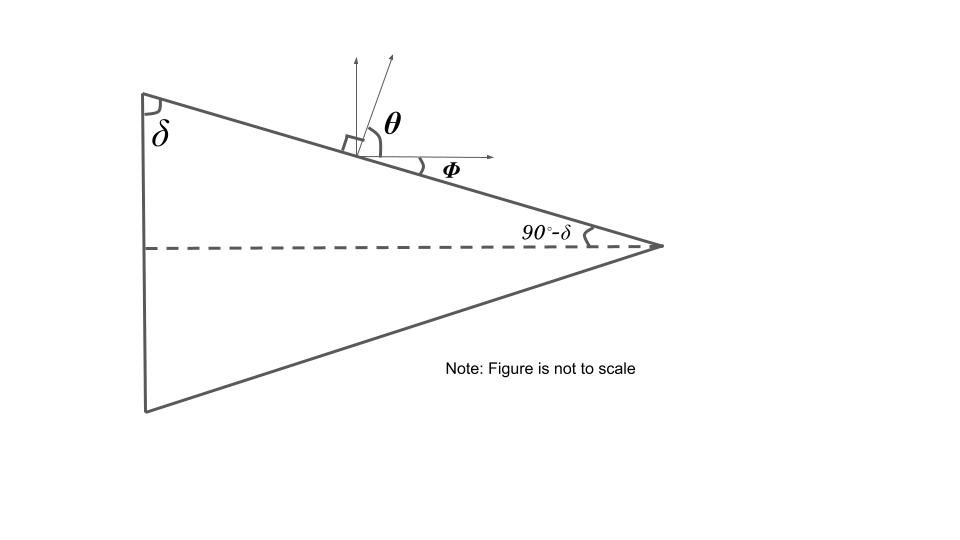
\includegraphics[width=0.99\textwidth]{javelin_dgm.jpg}
    \caption{One of the two cones of javelin, that contains the frontal area that we need to for the calculation of $k$}
    \label{fig:javelin_dgm.JPEG}
\end{figure}
Now, for frontal area, we can approximate as a pair of cones (of equal radius and height) stacked against each other, of radius 0.03 m \cite{ref8} and height 1.3 m \cite{ref9}. \\
As can be seen in the figure, and since they are alternate angles:
\begin{align}
    \phi = 90^\circ - \delta
\end{align}
Also, as can be seen in the figure:
\begin{align}
    \theta + \phi = 90^\circ
\end{align}
Now, substituting (24) into (25), we get
\begin{align}
    \theta = \delta
\end{align}
Now, from the figure, 
\begin{align*}
    \tan\delta &= \frac{1.3}{0.03} \\
    \delta &= \tan^{-1}\left(\frac{1.3}{0.03}\right) \\
    \delta &= 88.68^\circ \\
\end{align*}
Area of cone: Let the area of the cone be $A$
\begin{align*}
    A &= \pi*r*l \\
    &= \pi*r*\sqrt{r^2 + h^2} \\
    &= \pi*0.03*\sqrt{{0.03}^2 + {1.3}^2} \\
    &= \pi*0.03*\sqrt{1.6909} \\
    &= \pi*0.03*1.3 \\
    A &= 0.1225 \,m^2
\end{align*}
Now, since the frontal area is the exposed normally exposed area of the body, the magnitude of area exposed will be: $A\cos\theta$. And from (26), since $\delta = \theta$, we get the magnitude of area exposed to be: $A\cos\delta$. Therefore, the frontal area (say, $A_f$) is:
\begin{align*}
    A_f &= A*\cos\delta \\
    &= A\cos(88.68^\circ) \\
    &= 0.1225*0.002 \\
    A_f &= 0.003 m^2
\end{align*}
Therefore, we get the value of $k$ to be:
\begin{align*}
    k &= \frac{1}{2}*\rho_{air}*C*Frontal Area\\
    k &= 0.5*1.2\,kg/m^3*2.5*0.003\,m^2 \\
    k &= 0.00470625\,kg/m
\end{align*}
And, this value of $k$ is what we have given into the program
\newpage
%%%%%%%%%%%%%%%%%%%%%%%%%%%%%%%%%%%%%%%%%%%%%%%%
\section{Contribution of team mates}
\large{\bf {Contribution of {\it Lucky Upadhayay}}}
\begin{itemize}
   \item \textbf{In Formulation of the problem:} Computed the value of $k$, coefficient of friction for javelin 
   \item  \textbf{In Programming:} Made an integrated programme which saves data into output files, and wrote code for Euler method
   \item  \textbf{In Plotting Graphs:} Wrote GNU plot scripts for plotting the variation of $x_{max}$ with $\theta$, computed using all the 3 methods, and used EPS\LaTeX \space to produce the graphs in \LaTeX \space document
   \item  \textbf{In Report Writing:} Wrote abstract, introduction, and summary of the report, and combined the report. 
\end{itemize}
\large{\bf {Contribution of {\it Anurag Das}}}
\begin{itemize}
   \item \textbf{In Formulation of the problem:} Formulated the differential equation to be fed into the program
   \item  \textbf{In Programming:} Wrote code for the algorith for RK2 and RK4 methods
   \item  \textbf{In Plotting Graphs:} Wrote GNU plot script for the plotting the trajectories of the javelin thrown with various initial angles, and the "team10\_gnuscript.txt" file.
   \item  \textbf{In Report Writing:} Wrote the methodology and theory section of the report.
\end{itemize}
\large{\bf {Note: Inputs for the {\it Analysis of numerical results} section were equal from both the students.}}
%%%
\end{document}
